\chapter{Numerical results for the implicit coupling schemes}

This chapter provides validation and comparison results for most of the implicit solution schemes discussed in Chapter~\ref{chapter:implicit_meth}.
The methods considered are the fixed-point method (see Section~\ref{sec:fixed_point_approach}), the underrelaxation method (see Section~\ref{sec:underrelaxation}), the Aitken relaxation (see Section~\ref{sec:aitken_relaxation}), the Broyden-like family of methods, including Broyden's method (see Section~\ref{sec:multisecant}), the Newton-GMRES method (see Section~\ref{sec:newton_krylov}) and the polynomial vector extrapolation methods, MPE and RRE, in cycling mode (see Section~\ref{sec:vector_extrapolation}).
The use of predictors is also considered (see Section~\ref{sec:predictor}) as a way to improve efficiency.
It focuses on two thermomechanical examples for which reference solutions are available in the literature: the quasi-static finite strain thermo-elastic expansion of an infinitely long-thick walled cylinder and the necking of a thermo-elastoplastic circular bar.

% \section{Second Danilovskaya problem}
%
% The second Danilovskaya problem is proposed in \cite{danilovskaya_dynamical_1952} and it is used frequently in the literature for the validation of a fully coupled thermomechanical model (\cite{farhat_unconditionally_1991}, \cite{tosaka_boundary_1991}, \cite{tamma_effective_1992}, \cite{tanaka_application_1995} and \cite{danowski_computational_2014}).
% Following the description in \cite{danowski_computational_2014}, the geometry is in the form of a cuboid of height and width equal to \SI{4}{\milli\meter} and a length of \SI{6}{\milli\meter}, as is shown in Figure~\ref{fig:setup_2nd_danilovskaya}.
% The solid is linearly elastic and subject to a heat flux on the surface \(x=\SI{0}{\milli\meter}\).
% Here, \(\hat Q_C \equiv \hat q_C\) \jvc{Make notation consistent.} as only small deformation, i.e., \(\mathbf F \equiv \mathbf I\), are considered.
%
% \begin{figure}
%   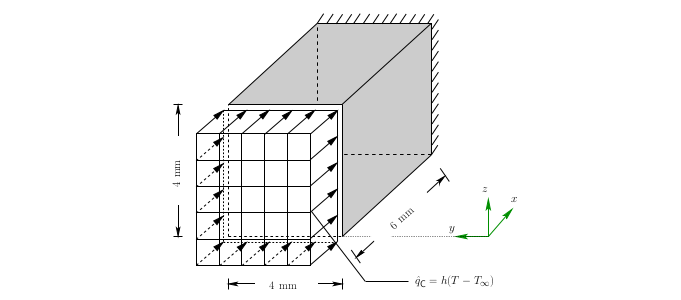
\includegraphics[width=.85\textwidth]{figures/setup_2nd_danilovskaya.png}
%   \caption{Setup for the second Danilovskaya problem. Initial geometry and prescribed heat convection boundary condition \(\hat q_C\).}
%   \label{fig:setup_2nd_danilovskaya}
% \end{figure}
%
% The simulation was performed in three spatial dimensions.
% However, all displacement degrees of freedom in the \(y\)- and \(z\)-directions are fixed, such that a quasi-one-dimensional motion is produced.
% The body is assumed to be mechanically constrained and thermally insulated.
%
% The mechanical and thermal field properties are given in Table~\ref{tab:snd_danilovskaya_description}, where \(\bar{h}\) denotes the kinematic heat transfer coefficient, defined as \(\bar{h}=\frac{h}{\rho C_V}\) with the linear heat transfer coefficient \(h\).
% Furthermore, the values for the thermal conductivity \(k\), the coefficient of thermal expansion \(\alpha_{T}\), the constant initial temperature \(T_{0}\), as well as an ambient temperature \(T_{\infty}\) are given.
% The elastic constants characterizing the material are Young's modulus \(E\) and Poisson's rate \(v\).
% A linear thermoelastic material is chosen according to the model described in \cite{armero_new_1992}.
%
% In the literature (\cite{farhat_unconditionally_1991}, \cite{tosaka_boundary_1991}, \cite{tamma_effective_1992}, \cite{tanaka_application_1995}), the density \(\rho\) and the heat capacity \(C_V\) are not divulged, and can in theory, be chosen arbitrarily according a dimensionless termomechanical parameter \(\delta\).
% However, to achieve a direct comparison with the results in \cite{tanaka_application_1995}, \cite{danowski_computational_2014} chose after calibration \(\rho=\SI{7.850}{\kilo\gram\meter^{-3}}\), yielding \(C_V = \SI[exponent-mode=engineering]{0.821}{\joule\kg^{-1}\kelvin^{-1}}\).
% These values are adopted here as well.
%
% \begin{table}
%   \centering
%   \caption{Material properties, and initial and boundary conditions for the second Danilovskaya problem.}
%   \label{tab:snd_danilovskaya_description}
%   \begin{tabular}{ccS[exponent-mode=engineering]}
%   \multicolumn{2}{c}{Material Properties} & {\vphantom{\Big |}Effective value}\\
%   \hline\hline
%   \vphantom{\Big |}Density \(\rho\) & (\si{\newton\second^2\milli\meter^{-4}}) & 7850e-12\\
%   \vphantom{\Big |}Young's modulus \(E\) & (\si{\newton\milli\meter^{-2}}) & 210e3\\
%   \vphantom{\Big |}Poisson's coefficient \(\nu\) & - & 0.3\\
%   \vphantom{\Big |}Conductivity \(k\) & (\si{\newton\second^{-1}\kelvin^{-1}}) & 1.03\\
%   \vphantom{\Big |}Heat capacity \(C_V\) & (\si{\milli\meter^2\second^{-2}\kelvin^{-1}}) & 0.821e6\\
%   \vphantom{\Big |}\makecell[c]{Coefficient of\\ thermal expansion} \(\alpha_T\) & (\si{\kelvin^{-1}}) & 1.1e-6\\
%   \hline
%   \multicolumn{2}{c}{Boundary Conditions\vphantom{\Big |}} & \\\hline
%   \vphantom{\Big |}Dimension \(l_x\) & (\si{\milli\meter}) & 6\\
%   \vphantom{\Big |}Dimension \(l_y\) & (\si{\milli\meter}) & 4\\
%   \vphantom{\Big |}Dimension \(l_z\) & (\si{\milli\meter}) & 4\\
%   \makecell[c]{Kinetic heat\\ convection coefficient} \(\bar h\) & (\si{\milli\meter\second^{-1}}) & 100e-3\\
%   \multicolumn{3}{c}{\vphantom{\Big |}All mechanical degrees of freedom fixed in the \(y\)- and \(z\)-directions.}\\
%   \hline
%   \multicolumn{2}{c}{Initial Conditions\vphantom{\Big |}} & \\\hline
%   \vphantom{\Big |}Ambient temperature \(T_\text{env}\) & (\si{\kelvin}) & {373.15}\\
%   Initial temperature \(T_0\) & (\si{\kelvin}) & {273.15}\\
%   \hline
%   \multicolumn{2}{c}{Reference value \vphantom{\Big |}} & \\\hline
%   \vphantom{\Big |}Temperature at point \(E\) (\(x=\SI{1}{\milli\meter}\)) & (\si{\kelvin}) & \\
%   \hline\hline
%   \end{tabular}
% \end{table}
%
% The discretisation for both the mechanical and thermal field contains each \(n_{x} \times n_{y} \times n_{z}=12 \times\) \(4 \times 4\) Hex 8 elements.
% The simulation time is \(t=\SI{4}{\second}\), with a time-step size of \(\Delta t=\SI{0.001}{\second}\).
% Moreover, a one-step- \(\theta\) time integration is chosen with the value \(\theta=0.5\), resulting in a CrankNicolson scheme for the temperature field and quasi-static approach for the mechanical field.
% Displacements and temperatures are evaluated at the center point of the plane at \(x=\SI{1}{\milli\meter}\).

\section{Expansion of a thermoelastic thick-walled cylinder}

The following numerical example concerns the quasi-static finite strain thermo-elastic expansion of an infinitely long thick-walled cylinder, as presented in \cite{ibrahimbegovic_thermodynamics_2009}.
\cite{armero_new_1992} and \cite{erbts_accelerated_2012} also present results regarding this problem, although the dimensions of the cylinder considered there are different from the ones used in the current work.
The example is comprised of an infinitely long cylinder with an inner radius of \(r_{0}=\SI{5}{\milli\meter}\) and an outer radius of \(r_{1}=\SI{15}{\milli\meter}\).
A displacement-driven problem is produced by enforcing an increasing radial displacement at the inner radius with a constant rate of \(\dot{u}_{0}\).
Following \cite{ibrahimbegovic_thermodynamics_2009}, the maximum displacement is set to \SI{10}{\milli\meter}, which clearly involves large deformations.
Zero heat flux is imposed at the inner radius, whereas the temperature at the outer radius is set to a reference temperature \(T_{0}\).
The initial temperature of the cylinder is also \(T_0\).
A sketch of the problem, including the initial and boundary conditions described, is shown in Figure~\ref{fig:problem_description}.
A decoupled Neo-Hookean free energy function characterizes the thermo-elastic material considered in this analysis, following \cite{armero_new_1992}.
Table~\ref{tab:expansion_thick_walled_cylinder} contains all material and model properties of relevance.

\begin{figure}[htbp]
 \centering
 \def\svgwidth{1.0\linewidth}
 \footnotesize
 \input{figures/thick_cylinder_problem_description.pdf_tex}
 \caption{Initial and boundary conditions considered in the quasi-static finite strain thermo-elastic expansion of an infinitely long thick-walled cylinder, and corresponding FEM mesh (QUAD4) used.}
\label{fig:problem_description}
\end{figure}

\begin{table}
 \centering
 \caption{Material properties and initial and boundary conditions for the problem concerning the quasi-static finite strain thermo-elastic expansion of an infinitely long thick-walled cylinder.}
\label{tab:expansion_thick_walled_cylinder}
 \begin{tabular}{lccS[exponent-mode=engineering]}
 \multicolumn{3}{c}{Material Properties} & {\vphantom{\Big |}Effective value}\\
 \hline\hline
 \vphantom{\Big |}Density & \(\rho\) & (\si{\newton\second^2\milli\meter^{-4}}) & 7.8e-9\\
 \vphantom{\Big |}Bulk modulus & \(\kappa\) & (\si{\newton\milli\meter^{-2}}) & 164206\\
 \vphantom{\Big |}Shear modulus & \(\mu\) & (\si{\newton\milli\meter^{-2}}) & 80140\\
 \vphantom{\Big |}Conductivity & \(k\) & (\si{\newton\second^{-1}\kelvin^{-1}}) & 45\\
 \vphantom{\Big |}Heat capacity & \(C_V\) & (\si{\milli\meter^2\second^{-2}\kelvin^{-1}}) & 460e6\\
 \vphantom{\Big |}Coefficient of thermal expansion & \(\alpha_T\) & (\si{\kelvin^{-1}}) & {\SI[exponent-mode=engineering]{0}{} - \SI[exponent-mode=engineering]{1.5e-4}{}}\\
 \hline
 \multicolumn{3}{c}{Boundary Conditions\vphantom{\Big |}} & \\\hline
 \vphantom{\Big |}Inner radius & \(r_0\) & (\si{\milli\meter}) & 5\\
 \vphantom{\Big |}Outer radius & \(r_1\) & (\si{\milli\meter}) & 15\\
 \vphantom{\Big |}Inner radius rate of displacement & \(\dot u_0\) & (\si{\milli\meter\second^{-1}}) & {0.1; 0.25; 0.5}\\
 \vphantom{\Big |}Heat at inner radius & \(q_1\) & (\si{\newton\second^{-1}\milli\meter^{-1}}) & 0\\
 \vphantom{\Big |}Temperature outer radius & \(T_1\) & (\si{\kelvin}) & 273.15\\
 % \multicolumn{3}{c}{\vphantom{\Big |}All mechanical degrees of freedom fixed in the \(y\)- and \(z\)-directions.}\\
 \hline
 \multicolumn{3}{c}{Initial Conditions\vphantom{\Big |}} & \\\hline
 Initial temperature & \(T_0\) & (\si{\kelvin}) & {273.15}\\
 \hline
 \multicolumn{3}{c}{Reference value \vphantom{\Big |}} & \\\hline
 \vphantom{\Big |}Temperature at inner radius (\(r=r_0\)) & (\si{\kelvin}) & \\
 \hline\hline
 \end{tabular}
\end{table}

A plane strain analysis is used to solve the problem, implying a null displacement and heat flux in the axial direction.
Linear quadratic elements (QUAD4) are used in the FEM discretization employed.
Thanks to the axial symmetry of the problem, only one-fourth of the cylinder is considered, as depicted in Figure~\ref{fig:problem_description}.
Except when explicitly indicated, the mesh employed contains 2601 nodes and 2500 elements.

The displacement is imposed in 200 equal time steps $\Delta t = \SI{0.1}{\second}$,
A quasi-static solution is computed for the mechanical problem using a backward Euler integration scheme. The transient temperature field is integrated in time employing the generalised-$\alpha$ method with $\rho_{\infty, T}=1.0$.

\subsection{Validation of the Numerical Results}

To validate the results presented in this work regarding the quasi-static finite strain thermo-elastic expansion of an infinitely long thick-walled cylinder, the problem is solved considering an \(\alpha_T = \SI{1.65e-4}{\kelvin^{-1}}\) and a \(\alpha_T = \SI{1.65e-5}{\kelvin^{-1}}\), at three different displacement rates for the inner radius, (\(\dot u_0 = \SIlist{0.1; 0.25; 0.5}{\milli\meter\second^{-1}}\)).
Reference results for this problem configuration are available in \cite{ibrahimbegovic_thermodynamics_2009} and provide a suitable comparison for validating the results obtained in the present work.
There is however one caveat, since in \cite{ibrahimbegovic_thermodynamics_2009} the results reported are supposedly for coefficients of thermal expansion equal to \SI{e-5}{\kelvin^{-1}} and \SI{e-4}{\kelvin^{-1}}.
The values used in the present work lead to the best fit between the present and the reference results.
The values chosen for the expansion coefficient lead to weak and strong coupling.
Using the latter value for the thermal expansion coefficient leads to instabilities when using a fixed-point explicit or implicit scheme with the isothermic split \citep{ibrahimbegovic_thermodynamics_2009, erbts_accelerated_2012}.

The temperature evolutions as a function of inner raidus displacement for a point located at the inner radius of the cylinder are presented in Figures~\ref{fig:thick_cylinder_validation_inner_radius_temperature_weak_coupled_quad4fbar} and \ref{fig:thick_cylinder_validation_inner_radius_temperature_strong_coupled_quad4fbar} chosing \(\alpha_T = \SI{1.65e-5}{\kelvin^{-1}}\) and \(\alpha_T =\SI{1.65e-4}{\kelvin^{-1}}\), respectively.
Figure~\ref{fig:thick_cylinder_temp_dist} presents the temperature distribution in half a transversal section of the thick-walled cylinder at increasing inner radius displacements.
A good agreement between the present work's numerical results and those found in \cite{ibrahimbegovic_thermodynamics_2009} can be observed for all displacement rates considered.
The temperature at the inner radius suffers a sharp decrease and then, as the displacement increases, tends to the reference temperature \(T_0\).
This decrease is due to the thermo-elastic heating effect and the fact that heat cannot be supplied from the outer radius fast enough to prevent this drop in temperature near the inner radius.

\begin{figure}[htbp]
 \centering
 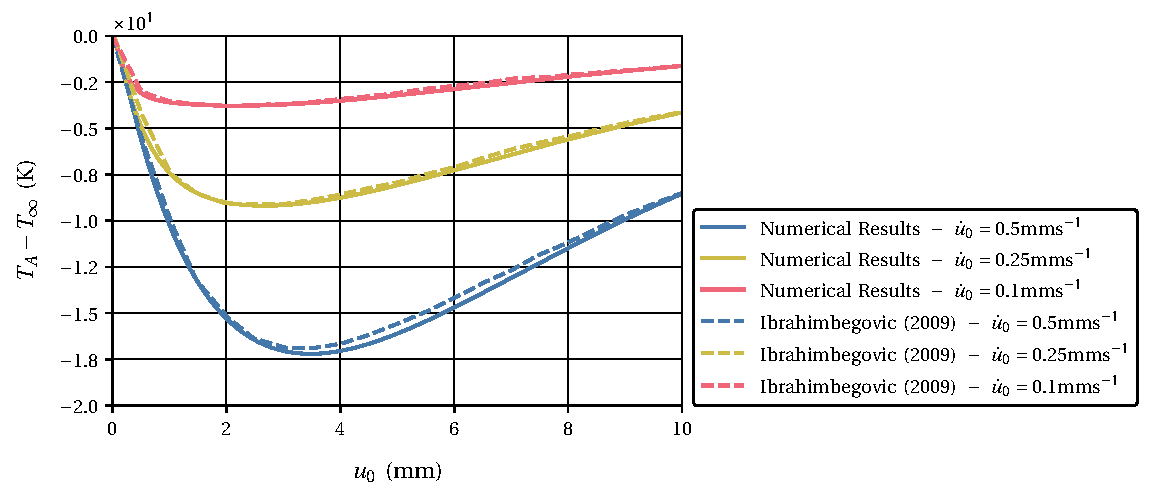
\includegraphics[width=.85\textwidth]{thick_cylinder_validation_inner_radius_temperature_weak_coupled_quad4fbar}
 \caption{Difference between the temperature at the inner radius and the reference temperature for the expansion of the thick-walled cylinder with \(\alpha_T=\SI{1.65e-5}{\kelvin^{-1}}\) and at different displacement rates for the inner radius (\(\dot u_0 = \SIlist{0.1; 0.25; 0.5}{\milli\meter\second^{-1}}\)}
\label{fig:thick_cylinder_validation_inner_radius_temperature_weak_coupled_quad4fbar}

\end{figure}
\begin{figure}[htbp]
 \centering
 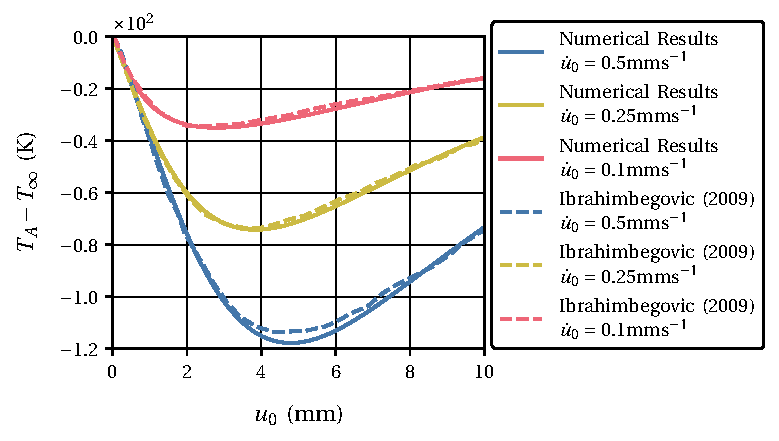
\includegraphics[width=.85\textwidth]{thick_cylinder_validation_inner_radius_temperature_strong_coupled_quad4fbar}
 \caption{Difference between the temperature at the inner radius and the reference temperature for the expansion of the thick-walled cylinder with \(\alpha_T=\SI{1.65e-4}{\kelvin^{-1}}\) and at different displacement rates for the inner radius (\(\dot u_0 = \SIlist{0.1; 0.25; 0.5}{\milli\meter\second^{-1}}\)}
\label{fig:thick_cylinder_validation_inner_radius_temperature_strong_coupled_quad4fbar}
\end{figure}

\begin{figure}[htbp]
 \centering
 \def\svgwidth{1.0\linewidth}
 \footnotesize
 \input{figures/thick_cylinder_temp_dist.pdf_tex}
 \caption{Temperature distribution in half a transversal section of the thick-walled cylinder at increasing inner radius displacements for \(\alpha_T=\SI{1.65e-4}{\kelvin^{-1}}\) and \(\dot u_0 = \SI{0.5}{\milli\meter\second^{-1}}\).}
\label{fig:thick_cylinder_temp_dist}
\end{figure}

\FloatBarrier

\subsection{Evaluation and comparison of implicit solution methods for the coupled problem}

The following contains the results concerning the evaluation and comparison of the implicit solution methods for coupled problems considered in this work.
The discussion starts with the methods that require only one evaluation of the residual per nonlinear iteration.
The Broyden-like family of methods fall into this category too but are considered by themselves and are presented next.
The Newton-Krylov methods are also analyzed, followed by the vector extrapolation methods in cycling mode.
The discussion ends with the comparison between the best methods in each class and the effect of predictors on the efficiency of the implicit methods.

The analysis presented is based mainly on three pieces of information.
The first concerns how the residual evolves as a function of the nonlinear iterations.
The second is the number of function evaluations needed to solve the coupled problem to the desired accuracy at each time step.
The third is the total number of residual evaluations needed to solve the coupled problem to the desired accuracy as a function of the thermal expansion coefficient.
The larger the thermal expansion coefficient, the stronger the coupling between the thermal and mechanical fields, and the more challenging the problem is to solve.
The evaluation of the residual implies the solution of the thermal and mechanical problems one after the other and takes the lion's share of computational time.
Regarding conclusions related to efficiency, it suffices when comparing methods of the same class to consider the number of residual evaluations.
The computational time is only analyzed in the comparison between the best methods of each class.

Only the displacement rate \(\dot u_0 = \SI{0.5}{\milli\meter\second^{-1}}\) is considered, with the thermal expansion coefficient varying from \SI{0}{\kelvin^{-1}} to \SI{1.5e-4}{\kelvin^{-1}}.

\subsubsection{Methods with only one residual evaluation per iteration}

The methods with only one residual evaluation per nonlinear iteration considered are the fixed-point method (see Section~\ref{sec:fixed_point_approach}), the underrelaxation method (see Section~\ref{sec:underrelaxation}), the Aitken relaxation (see Section~\ref{sec:aitken_relaxation}) and Broyden's method, Type I and II (see Section~\ref{sec:multisecant}).
These are, a priori, the most economical methods regarding residual evaluations, as only one is performed per nonlinear iteration.
The underrelaxation is performed with \(\omega = 0.5\), and the first relaxation coefficient for the Aitken relaxation is also set to 0.5.

Figure~\ref{fig:thick_cylinder_single_iter_residual_1st_time_step_quad4fbar_pred} presents the residual in percentage as a function of the number of nonlinear iterations in the first time step with \(\alpha_T=\SI{1.5e-4}{\kelvin^{-1}}\) and \(\dot u_0 =\SI{0.5}{\milli\meter\second^{-1}}\).
As reported by \cite{erbts_accelerated_2012}, the fixed-point scheme cannot converge for this thermal expansion coefficient value.
The other methods converge approximately linearly, with the Broyden and Aitken relaxation methods taking the same number of nonlinear iterations/residual evaluations.
Furthermore, the two Broyden methods are almost visually indistinguishable.
The underrelaxation methods take more iterations to converge, which
could be improved by tuning the relaxation coefficient further.

\begin{figure}[htbp]
 \centering
 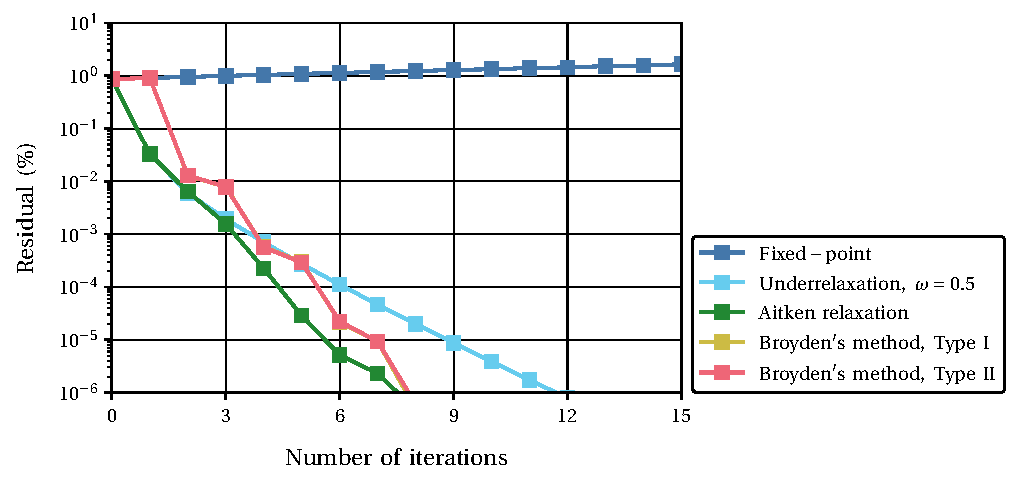
\includegraphics[width=.85\textwidth]{thick_cylinder_single_iter_residual_1st_time_step_quad4fbar_pred}
 \caption{Residual in percentage as a function of the number of nonlinear iterations in the first time step for the implicit methods that perform only one evaluation per nonlinear iteration in the solution of the quasi-static expansion of a thermoelastic thick-walled cylinder with \(\alpha_T=\SI{1.5e-4}{\kelvin^{-1}}\) and \(\dot u_0 =\SI{0.5}{\milli\meter\second^{-1}}\). }
\label{fig:thick_cylinder_single_iter_residual_1st_time_step_quad4fbar_pred}
\end{figure}

Figure~\ref{fig:thick_cylinder_single_iter_n_iter_time_quad4fbar_pred} presents the number of nonlinear iterations/residual evaluations needed to solve the coupled thermomechanical problem at each time step and the total (cumulative) number of iterations needed.
The strength of the coupling, tightly connected to the difficulty in solving the coupled problem and hence the number of nonlinear iterations needed to solve it, seems to be approximately uniform across the displacement range considered, with a slight decrease as the displacement increases.
The Broyden methods show a very similar behavior, besting the Aitken relaxation at each time step by at most one or two nonlinear iterations.
This leads to a sizable difference in the total number of function evaluations needed to solve the problem from start to finish.
The underrelaxation method underperforms again, showing even more difficulty in solving the problem as the displacement increases.

\begin{figure}[htbp]
 \centering
 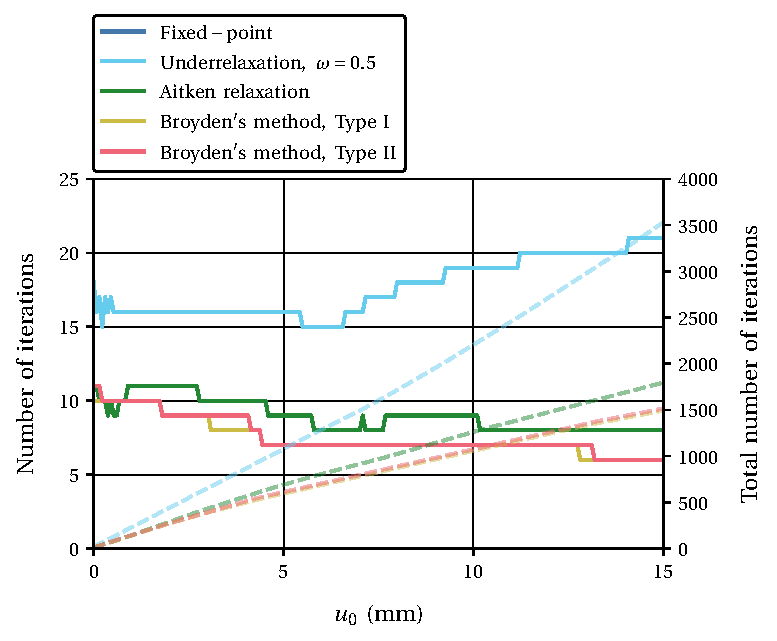
\includegraphics[width=.85\textwidth]{thick_cylinder_single_iter_n_iter_time_quad4fbar_pred}
 \caption{number of nonlinear iterations needed to solve the coupled problem at each time step and the total number of iterations needed to solve the coupled problem for the implicit methods that perform only one evaluation per nonlinear iteration  in the solution of the quasi-static expansion of a thermoelastic thick-walled cylinder with \(\alpha_T=\SI{1.5e-4}{\kelvin^{-1}}\) and \(\dot u_0 =\SI{0.5}{\milli\meter\second^{-1}}\).}
\label{fig:thick_cylinder_single_iter_n_iter_time_quad4fbar_pred}
\end{figure}

Figure~\ref{fig:thick_cylinder_single_iter_n_iter_coupl_strength_quad4fbar_pred} presents the total number of residual evaluations, in this case, corresponding also to the total number of nonlinear iterations, as a function of the thermal expansion coefficient, which controls the strength of the coupling between the thermal and the mechanical fields, respectively.
The residual evaluations correlate strongly with the total CPU time, accounting for the most significant portion of the computational time.
The most efficient methods are the two Broyden methods, followed by the Aitken relaxation.
The underrelaxation method performs poorly throughout the range of values considered for the thermal expansion coefficient, and the fixed-point becomes increasingly slow as the coupling gets stronger, eventually failing to converge for \(\alpha_T=\SI{1.5e-4}{\kelvin^{-1}}\).

\begin{figure}[htbp]
 \centering
 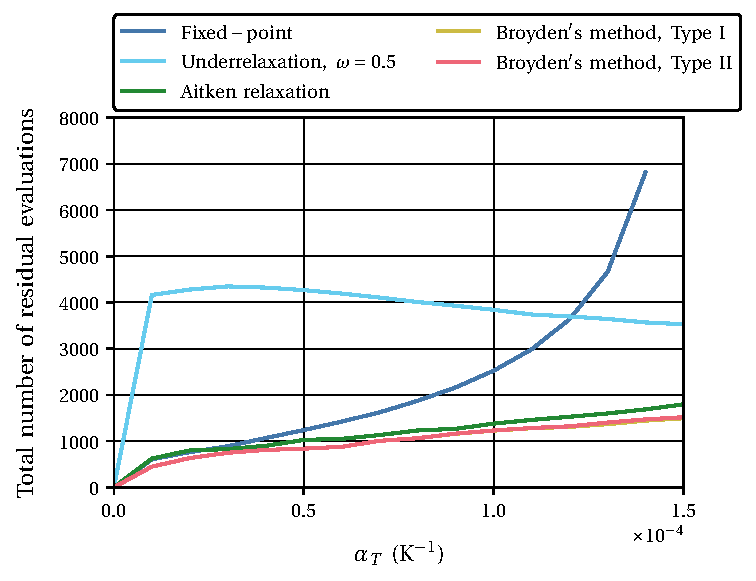
\includegraphics[width=.85\textwidth]{thick_cylinder_single_iter_n_iter_coupl_strength_quad4fbar_pred}
 \caption{Total number of residual evaluations as a function of the thermal expansion coefficient for the implicit methods that perform only one evaluation per nonlinear iteration in the solution of the quasi-static expansion of a thermoelastic thick-walled cylinder with \(\alpha_T=\SIrange{0}{1.5e-4}{\kelvin^{-1}}\) and \(\dot u_0 =\SI{0.5}{\milli\meter\second^{-1}}\).}
\label{fig:thick_cylinder_single_iter_n_iter_coupl_strength_quad4fbar_pred}
\end{figure}

\FloatBarrier

\subsubsection{Broyden-like method}

The Broyden-like methods considered (see Section~\ref{sec:multisecant}) employ as group sizes \(s=1,\ 2,\ 3,\ 6\) with a maximum number of previous iterations available equal to 6.
The mixing parameters considered are \(\beta=-1,\ \num{2e-3},\ \num{2e-2}\).
Their choice is based on prior tuning, which was not exhaustive.
All combinations are also considered with both Type I and Type II updating for the approximation to the Jacobian.

Figures~\ref{fig:thick_cylinder_broyden_like_type_i_residual_1st_time_step_quad4fbar_pred} and \ref{fig:thick_cylinder_broyden_like_type_ii_residual_1st_time_step_quad4fbar_pred} present the residual in percentage as a function of the number of nonlinear iterations in the first time step with \(\alpha_T=\SI{1.5e-4}{\kelvin^{-1}}\) and \(\dot u_0 =\SI{0.5}{\milli\meter\second^{-1}}\) for Broyden-like methods with Type I and Type II updates, respectively.
There is no marked difference between methods that employ a Type I and Type II update.
However, the choice of the mixing parameter and the group size leads to different behaviors for the residual.
For \(\beta=-1\), the methods using \(s=1\), 2, and 3 behave much the same with an approximately linear convergence rate and need the fewest iterations to reach the desired accuracy.
For \(s=6\), the residual behaves differently, plateauing for several nonlinear iterations.
Despite this, it only takes a few more iterations to converge when compared with the methods employing \(s=1\), 2, and 3.
When \(\beta=\num{2e-3}\) and \num{2e-2} are utilized, they exihibt a similar trend, with residual plateuas for a few iterations before decreasing.
This behavior can partly be explained by the implementation, which follows the suggestion found in \cite{fang_two_2009}.
Due to memory concerns, the approximation to the inverse of the Jacobian is only updated after the next group of residual evaluations has been filled (see Section~\ref{sec:multisecant}).
This approach can lead to a momentaneous poor approximation to the inverse of the Jacobian and thus stagnation of the residual.
The choice of \(\beta=\num{2e-2}\) seems to lead to slightly fewer iterations before the desired accuracy is reached.

\begin{figure}[htbp]
 \centering
 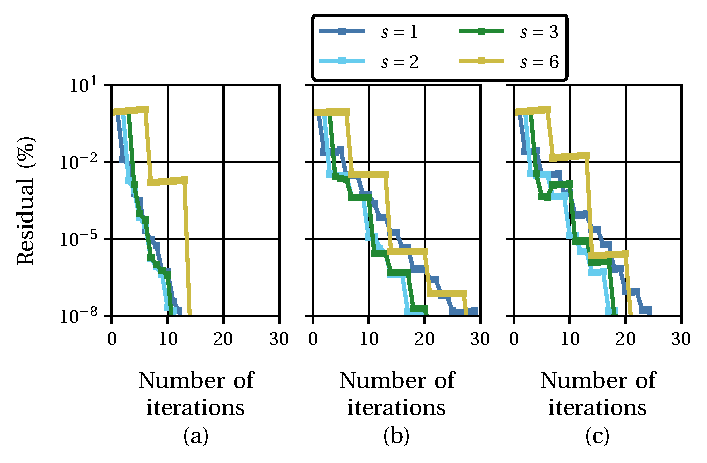
\includegraphics[width=.85\textwidth]{thick_cylinder_broyden_like_type_i_residual_1st_time_step_quad4fbar_pred}
 \caption{Residual in percentage as a function of the number of nonlinear iterations in the first time step for Broyden-like methods with Type I update and group sizes \(s=1\), 2, 4 and 6: (a) \(\beta=-1\), (b) \(\beta=\num{2e-3}\), and (c) \(\beta=\num{2e-2}\) in the solution of the quasi-static expansion of a thermoelastic thick-walled cylinder with \(\alpha_T=\SI{1.5e-4}{\kelvin^{-1}}\) and \(\dot u_0 =\SI{0.5}{\milli\meter\second^{-1}}\).}
\label{fig:thick_cylinder_broyden_like_type_i_residual_1st_time_step_quad4fbar_pred}
\end{figure}

\begin{figure}[htbp]
 \centering
 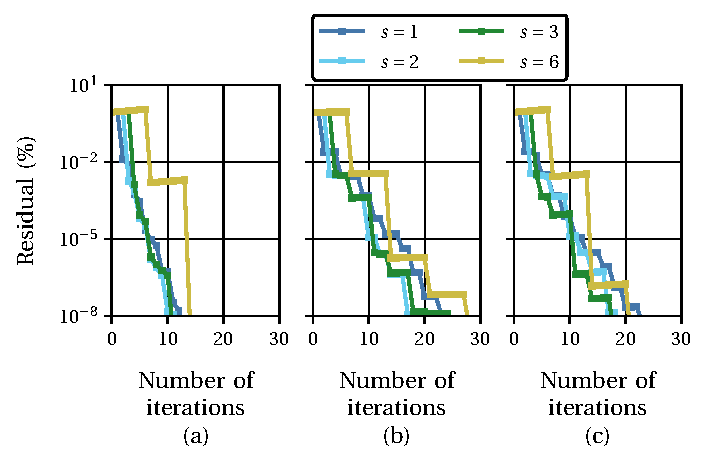
\includegraphics[width=.85\textwidth]{thick_cylinder_broyden_like_type_ii_residual_1st_time_step_quad4fbar_pred}
 \caption{Residual in percentage as a function of the number of nonlinear iterations in the first time step for Broyden-like methods with Type II update and group sizes \(s=1\), 2, 4 and 6: (a) \(\beta=-1\), (b) \(\beta=\num{2e-3}\), and (c) \(\beta=\num{2e-2}\) in the solution of the quasi-static expansion of a thermoelastic thick-walled cylinder with \(\alpha_T=\SI{1.5e-4}{\kelvin^{-1}}\) and \(\dot u_0 =\SI{0.5}{\milli\meter\second^{-1}}\).}
\label{fig:thick_cylinder_broyden_like_type_ii_residual_1st_time_step_quad4fbar_pred}
\end{figure}

Figures~\ref{fig:thick_cylinder_broyden_like_type_i_n_iter_time_quad4fbar_pred} and \ref{fig:thick_cylinder_broyden_like_type_ii_n_iter_time_quad4fbar_pred} present the number of nonlinear iterations/number of function evaluations needed to solve the coupled problem at each time step and the total (cumulative) number of iterations needed.
Again the differences between the Broyden-like methods using Type I and Type II updates are not pronounced.
Perhaps the most noticeable difference is for \(\beta=\num{2e-3}\) and \num{2e-2}, where the total number of iterations needed to solve the coupled thermomechanical problem oscillates more strongly between time steps for the Type I methods.
For \(\beta=-1\), the methods using group sizes of 1, 2, and 3 display a higher efficiency, which disappears as the displacement increases.
For \(\beta=\num{2e-2}\) and \num{2e-3}, the results seem to indicate the need for fewer iterations when using group sizes of 2 and 3.

\begin{figure}[htbp]
 \centering
 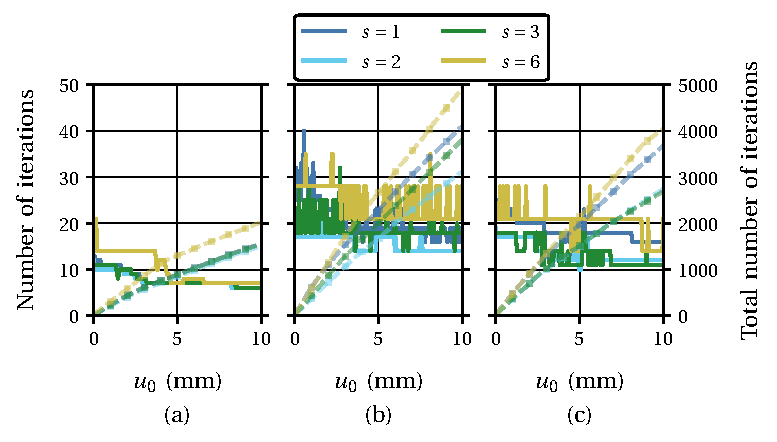
\includegraphics[width=.85\textwidth]{thick_cylinder_broyden_like_type_i_n_iter_time_quad4fbar_pred}
 \caption{Number of nonlinear iterations needed to solve the coupled problem at each time step and the total number of iterations needed to solve the coupled problem for Broyden-like methods with Type I update and group sizes \(s=1\), 2, 4 and 6: (a) \(\beta=-1\), (b) \(\beta=\num{2e-3}\), and (c) \(\beta=\num{2e-2}\) in the solution of the quasi-static expansion of a thermoelastic thick-walled cylinder with \(\alpha_T=\SI{1.5e-4}{\kelvin^{-1}}\) and \(\dot u_0 =\SI{0.5}{\milli\meter\second^{-1}}\).}
\label{fig:thick_cylinder_broyden_like_type_i_n_iter_time_quad4fbar_pred}
\end{figure}

\begin{figure}[htbp]
 \centering
 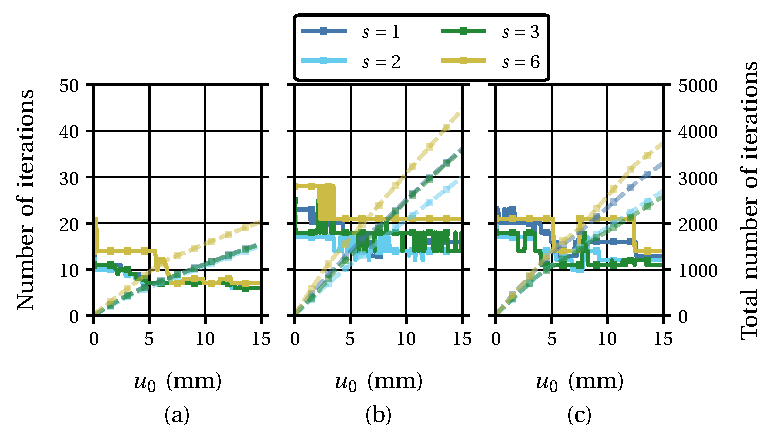
\includegraphics[width=.85\textwidth]{thick_cylinder_broyden_like_type_ii_n_iter_time_quad4fbar_pred}
 \caption{Number of nonlinear iterations needed to solve the coupled problem at each time step and the total number of iterations needed to solve the coupled problem for Broyden-like methods with Type II update and group sizes \(s=1\), 2, 4 and 6: (a) \(\beta=-1\), (b) \(\beta=\num{2e-3}\), and (c) \(\beta=\num{2e-2}\) in the solution of the quasi-static expansion of a thermoelastic thick-walled cylinder with \(\alpha_T=\SI{1.5e-4}{\kelvin^{-1}}\) and \(\dot u_0 =\SI{0.5}{\milli\meter\second^{-1}}\).}
\label{fig:thick_cylinder_broyden_like_type_ii_n_iter_time_quad4fbar_pred}
\end{figure}

Figures~\ref{fig:thick_cylinder_broyden_like_type_i_n_iter_coupl_strength_quad4fbar_pred} presents the total number of residual evaluations as a function of the thermal expansion coefficient, respectively, for the Broyden-like methods with Type I update considered.
The same results are presented in Figures~\ref{fig:thick_cylinder_broyden_like_type_ii_n_iter_coupl_strength_quad4fbar_pred} for the Broyden-like methos with Type II update.
The most efficient methods employ a mixing parameter equal to \(\beta=-1\) and group sizes equal to 1, 2, and 3.
The choices of \num{2e-3} and \num{2e-2} for the mixing parameter lead to less efficient methods, which need a more significant amount of residual evaluations and thus require more CPU time to solve the coupled thermomechanical problem completely.

\begin{figure}[htbp]
 \centering
 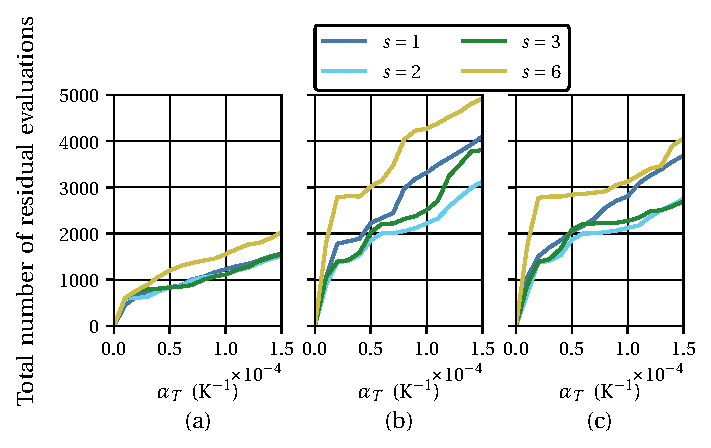
\includegraphics[width=.85\textwidth]{thick_cylinder_broyden_like_type_i_n_iter_coupl_strength_quad4fbar_pred}
 \caption{Total number of residual evaluations as a function of the thermal expansion coefficient for the implicit methods for Broyden-like methods with Type I update and group sizes \(s=1\), 2, 4 and 6: (a) \(\beta=-1\), (b) \(\beta=\num{2e-3}\), and (c) \(\beta=\num{2e-2}\) in the solution of the quasi-static expansion of a thermoelastic thick-walled cylinder with \(\alpha_T=\SIrange{0}{1.5e-4}{\kelvin^{-1}}\) and \(\dot u_0 =\SI{0.5}{\milli\meter\second^{-1}}\).}
\label{fig:thick_cylinder_broyden_like_type_i_n_iter_coupl_strength_quad4fbar_pred}
\end{figure}

\begin{figure}[htbp]
 \centering
 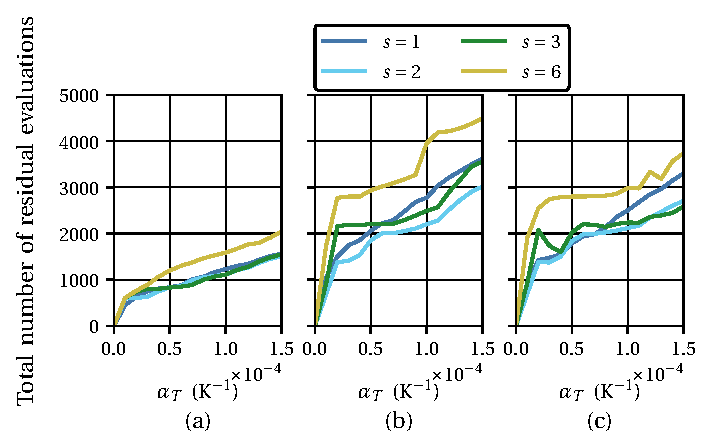
\includegraphics[width=.85\textwidth]{thick_cylinder_broyden_like_type_ii_n_iter_coupl_strength_quad4fbar_pred}
 \caption{Total number of residual evaluations as a function of the thermal expansion coefficient for Broyden-like methods with Type II update and group sizes \(s=1\), 2, 4 and 6: (a) \(\beta=-1\), (b) \(\beta=\num{2e-3}\), and (c) \(\beta=\num{2e-2}\) in the solution of the quasi-static expansion of a thermoelastic thick-walled cylinder with \(\alpha_T=\SIrange{0}{1.5e-4}{\kelvin^{-1}}\) and \(\dot u_0 =\SI{0.5}{\milli\meter\second^{-1}}\).}
\label{fig:thick_cylinder_broyden_like_type_ii_n_iter_coupl_strength_quad4fbar_pred}
\end{figure}

\FloatBarrier

\subsubsection{Newton-GMRES method}

The Newton-Krylov method examined here uses as the Krylov subspace solver the GMRES method (see Section~\ref{sec:newton_krylov}).
Different forcing terms are employed.
The values considered are \(\eta=\num[print-unity-mantissa=false]{e-1}\), \num[print-unity-mantissa=false]{e-3} and \num[print-unity-mantissa=false]{e-5}.
The Eisenstat-Walker scheme for the adaptive choice of the forcing term is also utilized.

Figure~\ref{fig:thick_cylinder_newton_krylov_residual_1st_time_step_quad4fbar_pred} presents the residual in percentage as a function of the number of nonlinear iterations in the first time step with \(\alpha_T=\SI{1.5e-4}{\kelvin^{-1}}\) and \(\dot u_0 =\SI{0.5}{\milli\meter\second^{-1}}\).
For \(\eta=\num{e-5}\), the Newton-GMRES method converges quadratically since the Newton system is solved to a finer accuracy, thus closely approximating the Newton-Raphson scheme.
As \(\eta\) increases, the convergence rate as a function of the number of nonlinear iterations slows down.
The method employing the Eisenstat-Walker scheme performs similarly to the method using a constant forcing term equal to \num{e-1}.
Keep in mind that within each nonlinear iteration, the Newton-Krylov methods may evaluate the function several times, such that converging in fewer nonlinear iterations does not necessarily imply a more efficient method regarding computational time spent solving the coupled thermomechanical problem.

\begin{figure}
 \centering
 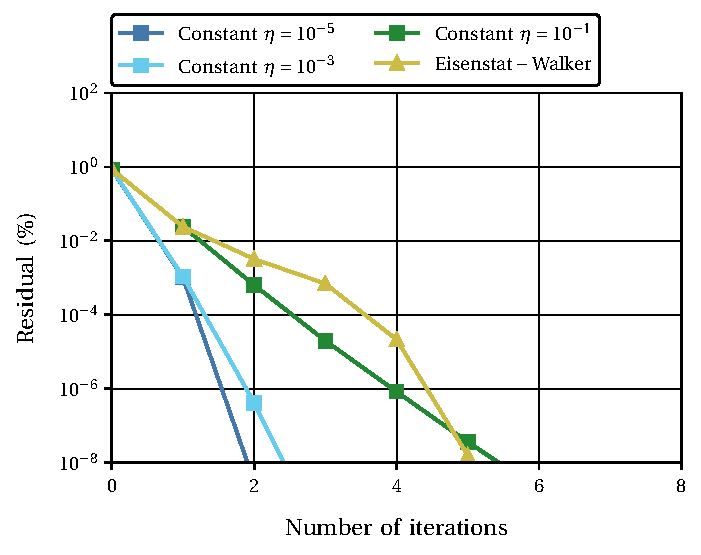
\includegraphics[width=.85\textwidth]{thick_cylinder_newton_krylov_residual_1st_time_step_quad4fbar_pred}
 \caption{Residual in percentage as a function of the number of nonlinear iterations in the first time step for the Newton-GMRES method with a constant forcing term (\(\eta=\num{1e-5},\ \num{1e-3},\ \num{1e-1}\)) and the Eisenstat-Walker scheme in the solution of the quasi-static expansion of a thermoelastic thick-walled cylinder with \(\alpha_T=\SI{1.5e-4}{\kelvin^{-1}}\) and \(\dot u_0 =\SI{0.5}{\milli\meter\second^{-1}}\).}
\label{fig:thick_cylinder_newton_krylov_residual_1st_time_step_quad4fbar_pred}
\end{figure}

Figure~\ref{fig:thick_cylinder_newton_krylov_n_iter_time_quad4fbar_pred} presents the number of nonlinear iterations needed to solve the coupled problem at each time step and the total (cumulative) number of iterations needed.
The strength of the coupling seems to be approximately uniform across the displacement range considered, as the number of iterations taken by each method remains approximately constant as the displacement increases.
As hinted by the results already discussed regarding the residual as a function of the nonlinear iterations in the first time step, the smaller the forcing, the fewer the number of nonlinear iterations needed to solve the coupled problem at each time step.
The method that uses the Eisenstat-Walker scheme performs similarly to the method using a constant forcing term equal to \num{1e-1}.

\begin{figure}
 \centering
 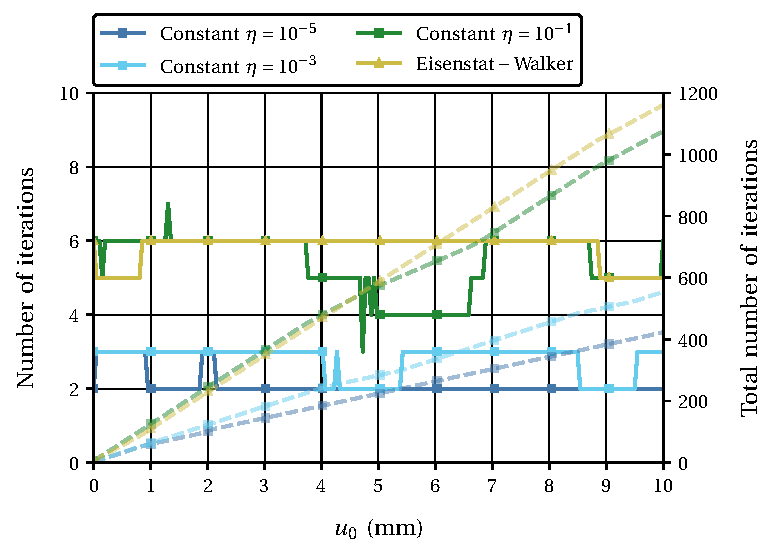
\includegraphics[width=.85\textwidth]{thick_cylinder_newton_krylov_n_iter_time_quad4fbar_pred}
 \caption{Number of nonlinear iterations needed to solve the coupled problem at each time step and the total number of iterations needed to solve the coupled problem for the Newton-GMRES method with a constant forcing term (\(\eta=\num{1e-5},\ \num{1e-3},\ \num{1e-1}\)) and the Eisenstat-Walker scheme in the solution of the quasi-static expansion of a thermoelastic thick-walled cylinder with \(\alpha_T=\SI{1.5e-4}{\kelvin^{-1}}\) and \(\dot u_0 =\SI{0.5}{\milli\meter\second^{-1}}\).}
\label{fig:thick_cylinder_newton_krylov_n_iter_time_quad4fbar_pred}
\end{figure}

Figures~\ref{fig:thick_cylinder_newton_krylov_n_iter_time_quad4fbar_pred} presents the total number of residual evaluations a function of the thermal expansion coefficient.
The most efficient Newton-GMRES methods analyzed are the ones using a constant forcing term equal to \num{1e-5} and \num{1e-3}, followed by the technique employing a constant forcing term equal to \num{1e-1} and then by the method utilizing the Eisenstat-Walker scheme.

\begin{figure}
 \centering
 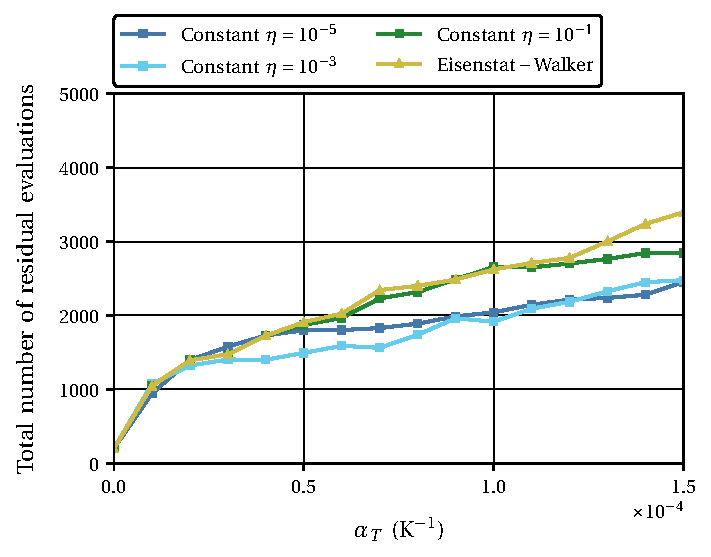
\includegraphics[width=.85\textwidth]{thick_cylinder_newton_krylov_n_iter_coupl_strength_quad4fbar_pred}
 \caption{Total number of residual evaluations as a function of the thermal expansion coefficient for the Newton-GMRES method with a constant forcing term (\(\eta=\num{1e-5},\ \num{1e-3},\ \num{1e-1}\)) and the Eisenstat-Walker scheme in the solution of the quasi-static expansion of a thermoelastic thick-walled cylinder with \(\alpha_T=\SIrange{0}{1.5e-4}{\kelvin^{-1}}\) and \(\dot u_0 =\SI{0.5}{\milli\meter\second^{-1}}\).}
\label{fig:thick_cylinder_newton_krylov_n_iter_coupl_strength_quad4fbar_pred}
\end{figure}

\FloatBarrier

\subsubsection{Polynomial vector extrapolation in cycling mode}

The polynomial vector extrapolation methods in cycling mode considered are the MPE and RRE, restricted to at most five evaluations of the residual function per nonlinear iteration.
Thus, the combinations analyzed are characterized by the ordered pairs \((n,k)=(1,1)\), \((1,2)\), \((1,3)\), \((2,1)\), \((2,2)\) and \((3,1)\) (see Section~\ref{sec:vector_extrapolation}).

Figure~\ref{fig:thick_cylinder_extrap_pol_residual_1st_time_step_quad4fbar_pred} presents the residual in percentage as a function of the number of nonlinear iterations in the first time step with \(\alpha_T=\SI{1.5e-4}{\kelvin^{-1}}\) and \(\dot u_0 =\SI{0.5}{\milli\meter\second^{-1}}\).
In general, the larger the number of residual evaluations per nonlinear iteration, the faster rate of convergence.
Also, it seems that for the same number of residual evaluations per nonlinear iterations, e.g., \((n,k)=(1,3)\), \((2,2)\) and \((3,1)\) or \((n,k)=(1,2)\), \((2,1)\), it is more profitable to increase \(k\) than \(n\).
The results for the MPE and the RRE are very similar.

\begin{figure}[htbp]
 \centering
 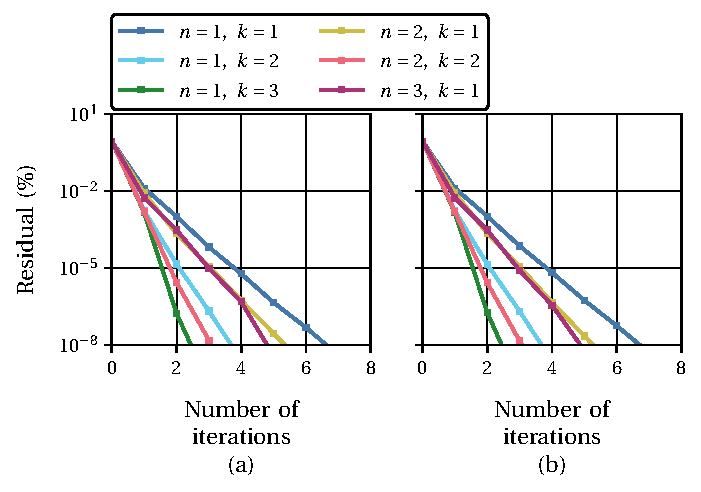
\includegraphics[width=0.9\textwidth]{thick_cylinder_extrap_pol_residual_1st_time_step_quad4fbar_pred}
 \caption{Residual in percentage as a function of the number of nonlinear iterations in the first time step for the polynomial vector extrapolation methods in cycling mode, MPE and RRE, restricted to at most five evaluations of the residual function per nonlinear iteration in the solution of the quasi-static expansion of a thermoelastic thick-walled cylinder with \(\alpha_T=\SI{1.5e-4}{\kelvin^{-1}}\) and \(\dot u_0 =\SI{0.5}{\milli\meter\second^{-1}}\).}
\label{fig:thick_cylinder_extrap_pol_residual_1st_time_step_quad4fbar_pred}
\end{figure}

Figure~\ref{fig:thick_cylinder_extrap_pol_n_iter_time_quad4fbar_pred} presents the number of residual evaluations needed to solve the coupled problem at each time step and the total (cumulative) number of iterations needed.
The number of nonlinear iterations needed to solve the coupled problem to the desired accuracy at each time step remains approximately constant, with a slight decrease as the displacement increases.
As before, the MPE and RRE methods display very similar performances.
As hinted by the previous results regarding the residual, the methods with more residual evaluations per nonlinear iteration take, in general, fewer iterations to converge.

\begin{figure}[htbp]
 \centering
 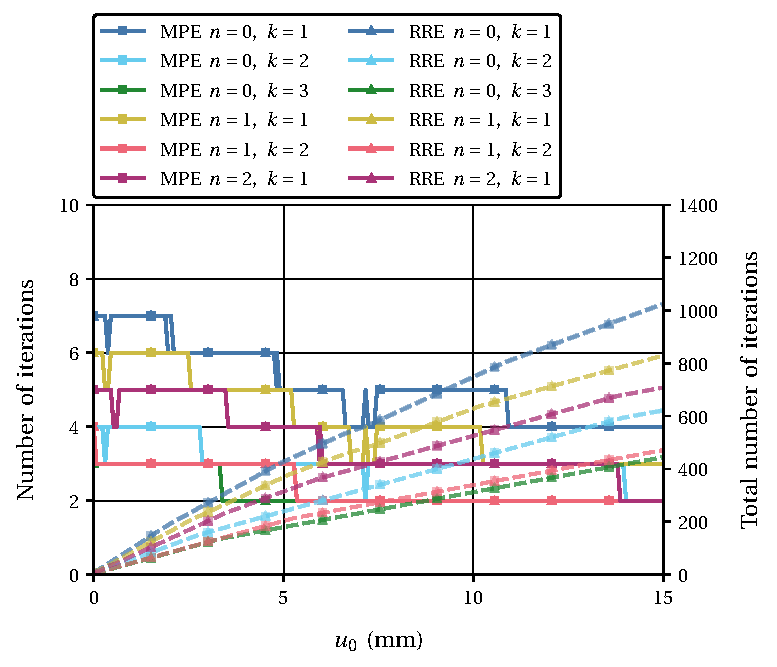
\includegraphics[width=0.9\textwidth]{thick_cylinder_extrap_pol_n_iter_time_quad4fbar_pred}
 \caption{number of nonlinear iterations needed to solve the coupled problem at each time step and the total number of iterations needed to solve the coupled problem for the polynomial vector extrapolation methods in cycling mode, MPE and RRE, restricted to at most five evaluations of the residual function per nonlinear iteration in the solution of the quasi-static expansion of a thermoelastic thick-walled cylinder with \(\alpha_T=\SI{1.5e-4}{\kelvin^{-1}}\) and \(\dot u_0 =\SI{0.5}{\milli\meter\second^{-1}}\).}
\label{fig:thick_cylinder_extrap_pol_n_iter_time_quad4fbar_pred}
\end{figure}

Figures~\ref{fig:thick_cylinder_extrap_pol_n_iter_time_quad4fbar_pred} presents the total number of residual evaluations as a function of the thermal expansion coefficient.
There is not a clear winner regarding the total number of residual evaluations taken to solve the coupled thermomechanical problem completely, but the methods with \((n,k)=(1,3)\), \((1,2)\) and \((2,2)\) seem to always be in the top spots regarding efficiency.

\begin{figure}[htbp]
 \centering
 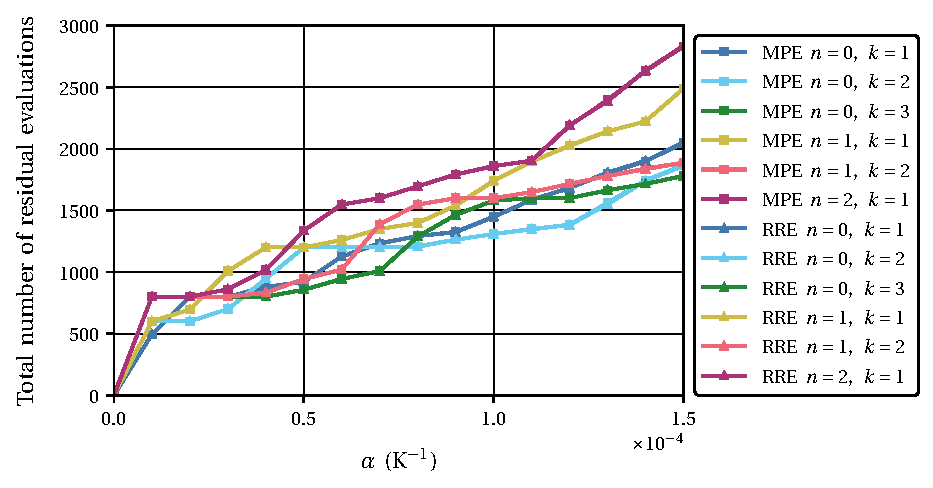
\includegraphics[width=0.9\textwidth]{thick_cylinder_extrap_pol_n_iter_coupl_strength_quad4fbar_pred}
 \caption{Total number of residual evaluations as a function of the thermal expansion coefficient for the polynomial vector extrapolation methods in cycling mode, MPE and RRE, restricted to at most five evaluations of the residual function per nonlinear iteration in the solution of the quasi-static expansion of a thermoelastic thick-walled cylinder with \(\alpha_T=\SIrange{0}{1.5e-4}{\kelvin^{-1}}\) and \(\dot u_0 =\SI{0.5}{\milli\meter\second^{-1}}\).}
\label{fig:thick_cylinder_extrap_pol_n_iter_coupl_strength_quad4fbar_pred}
\end{figure}

\FloatBarrier

\subsubsection{comparison of the best methods in each class}

In this section, the best-performing methods from each of the classes considered are compared with each other.
The implicit methods selected are the Aitken relaxation, Broyden's method with Type I update, a Broyden-like method with \(\beta=-1\) and \(s=2\), the Newton-GMRES method with \(\eta=\num{e-3}\) and the MPE in cycling mode with \((n,k)=(1,3)\).

Figure~\ref{fig:thick_cylinder_comparison_best_cpu_time_n_iter_coupl_strength_quad4fbar_pred} shows the total CPU time in seconds and the total number of residual evaluations as a function of the thermal expansion coefficient for the best performing implicit methods in each class considered.
The best performing methods are Broyden's method and the Broyden-like method with \(\beta=-1\), followed by the Aitken relaxation, the MPE in cycling mode, and the Newton-GMRES method.
As the thermal coefficient, and thus the strength of the coupling, increases, all the methods display a loss in efficiency.
Table~\ref{tab:res_cpu_nr_func_best} surmises all the results previously discussed regarding the computational time taken by each solver.

Figure~\ref{fig:thick_cylinder_comparison_best_time_profile_mesh_size_quad4fbar_pred} depicts the total CPU time in seconds, and time profile, as a function of the mesh size.
For all solvers and mesh sizes, evaluating the solvers is the operation that takes up the most computational time.
The computation of the residual function considered implies the solution of both the mechanical and thermal problems, with the mechanical solver taking longer than the thermal solver.
This difference can be partly explained because it has double the number of degrees of freedom.
Also, the operations concerning the constitutive behavior of the material are performed in the mechanical solver for the implementation developed in this work.
The time spent on operations concerning the coupling solver solely contributes a small weight to the total time for all mesh sizes and solvers.
This relative importance of the operations in the coupling solver is verified despite the volumetric coupling between the mechanical and thermal problems.
A volumetric coupling leads to all the degrees of freedom in one of the solvers, in this case, the thermal solver, to have to be considered by the coupling procedure.
In contrast, only the degrees of freedom at the contact surface need to be considered for surface coupling, such as the one found in fluid-structure interaction.

\begin{figure}[hbtp]
 \centering
 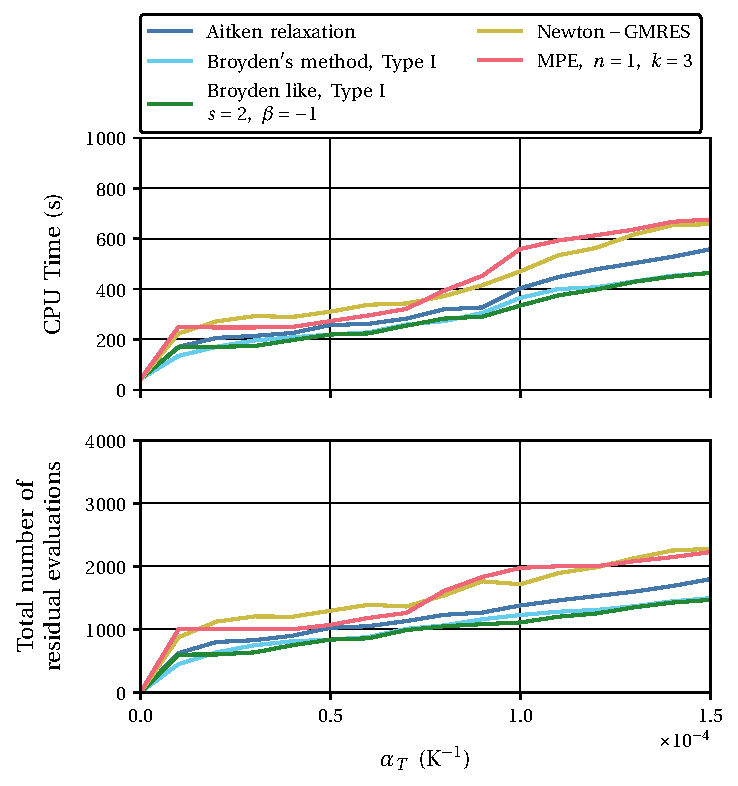
\includegraphics[width=.85\textwidth]{thick_cylinder_comparison_best_cpu_time_n_iter_coupl_strength_quad4fbar_pred}
 \caption{Total CPU time in seconds and the total number of residual evaluations as a function of the thermal expansion coefficient for the  best performing implicit methods in each class considered in the solution of the quasi-static expansion of a thermoelastic thick-walled cylinder with \(\alpha_T=\SIrange{0}{1.5e-4}{\kelvin^{-1}}\) and \(\dot u_0 =\SI{0.5}{\milli\meter\second^{-1}}\).}
\label{fig:thick_cylinder_comparison_best_cpu_time_n_iter_coupl_strength_quad4fbar_pred}
\end{figure}

\begin{table}[hbtp]
 \centering
 \caption{Total CPU time in seconds and total number of residual evaluations as a function of the thermal expansion coefficient for the  best performing implicit methods in each class considered in the solution of the quasi-static expansion of a thermoelastic thick-walled cylinder with \(\alpha_T=\SIlist{5e-5; 10e-5; 15e-5}{\kelvin^{-1}}\), and \(\dot u_0 =\SI{0.5}{\milli\meter\second^{-1}}\).}
 \label{tab:res_cpu_nr_func_best}
 % \setlength{\tabcolsep}{3pt}
 \begin{tabular}
 {l
 S[round-mode=places, round-precision=2, table-format = 1.2e1]
 S[round-mode=places, round-precision=2, table-format = 1.2e1]
 S[round-mode=places, round-precision=2, table-format = 1.2e1]
 S[round-mode=places, round-precision=0, exponent-mode=fixed, fixed-exponent=0, table-number-alignment = center, table-format = 4.0]
 S[round-mode=places, round-precision=0, exponent-mode=fixed, fixed-exponent=0, table-number-alignment = center, table-format = 4.0]
 S[round-mode=places, round-precision=0, exponent-mode=fixed, fixed-exponent=0, table-number-alignment = center, table-format = 4.0] }
 \vphantom{\Big \vert}&  \multicolumn{3}{c}{CPU Time (\si{\second})} & \multicolumn{3}{c}{Nr Residual Evaluations} \\
 \cmidrule(lr){2-4}\cmidrule(lr){5-7}
 \vphantom{\Big \vert}\makecell[c]{$\alpha_T$\\ (\SI[exponent-mode=input]{1e-5}{\kelvin^{-1}})} & {5} & {10} & {15} & {5} & {10} & {15}\\
 \hline\hline
 \vphantom{\Big \vert}  AITK  & 2.57200e2 & 4.03400e2 & 5.58200e2 & 1.02500e+03 & 1.37800e+03 & 1.79600e+03\\
 \vphantom{\Big \vert}  BRDI  & \cellcolor{gray}2.19600e+02 & 3.64900e+02 & \cellcolor{gray}4.64000e+02 & \cellcolor{gray}8.36000e+02 & 1.22600e+03 & 1.49400e+03\\
 \vphantom{\Big \vert}  BRDI2  & \cellcolor{gray}2.19700e+02 & \cellcolor{gray}3.34600e+02 & 4.64500e+02 & \cellcolor{gray}8.36000e+02 & \cellcolor{gray}1.10800e+03 & \cellcolor{gray}1.46600e+03\\
 \vphantom{\Big \vert}  NEWT  & 3.10500e+02 & 4.70500e+02 & 6.57600e+02 & 1.29400e+03 & 1.71400e+03 & 2.27700e+03\\
 \vphantom{\Big \vert}  MPE  & 2.73100e+02 & 5.59100e+02 & 6.76100e+02 & 1.07000e+03 & 1.97500e+03 & 2.22500e+03\\


 \hline\hline
 \end{tabular}
\end{table}

\begin{figure}[hbtp]
 \centering
 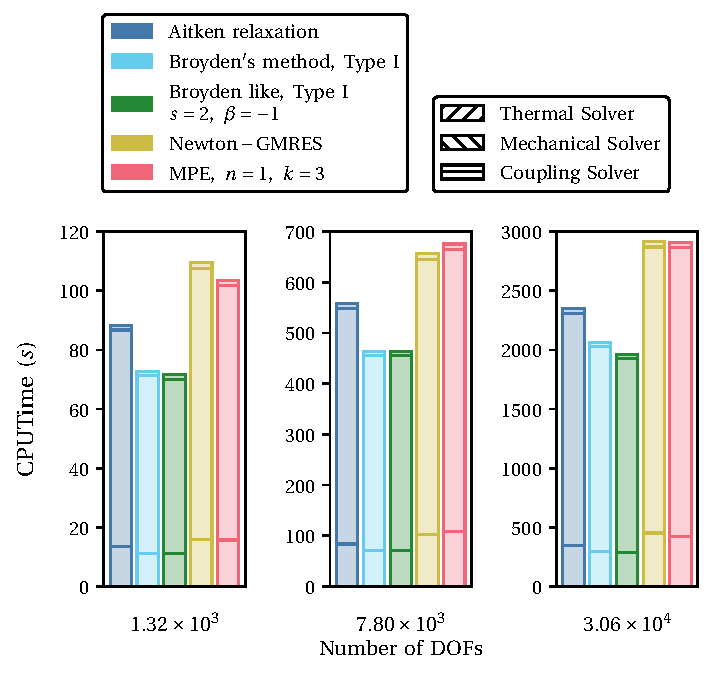
\includegraphics[width=.85\textwidth]{thick_cylinder_comparison_best_time_profile_mesh_size_quad4fbar_pred}
 \caption{Total CPU time in seconds, and time profile, as a function of the mesh size for the  best performing implicit methods in each class considered in the solution of the quasi-static expansion of a thermoelastic thick-walled cylinder with \(\alpha_T=\SI{1.5e-4}{\kelvin^{-1}}\) and \(\dot u_0 =\SI{0.5}{\milli\meter\second^{-1}}\).}
\label{fig:thick_cylinder_comparison_best_time_profile_mesh_size_quad4fbar_pred}
\end{figure}

\FloatBarrier

\subsubsection{Effect of predictiors}

Figure~\ref{fig:thick_cylinder_comparison_best_pred_total_iters_coupl_strength_quad4fbar_pred.pdf} presents the effect of employing a linear or quadratic predictor on the number of residual evaluations needed to fully solve the thermomechanical problem under analysis as a function of the thermal expansion coefficient.
All methods improve using the polynomial predictors, with the best results achieved using the quadratic predictor.
The decrease in the number of residual evaluations is around 30\% to 40\%.
Their effect seems to display a slight increase as the coupling gets stronger.

\begin{figure}[hbtp]
 \centering
 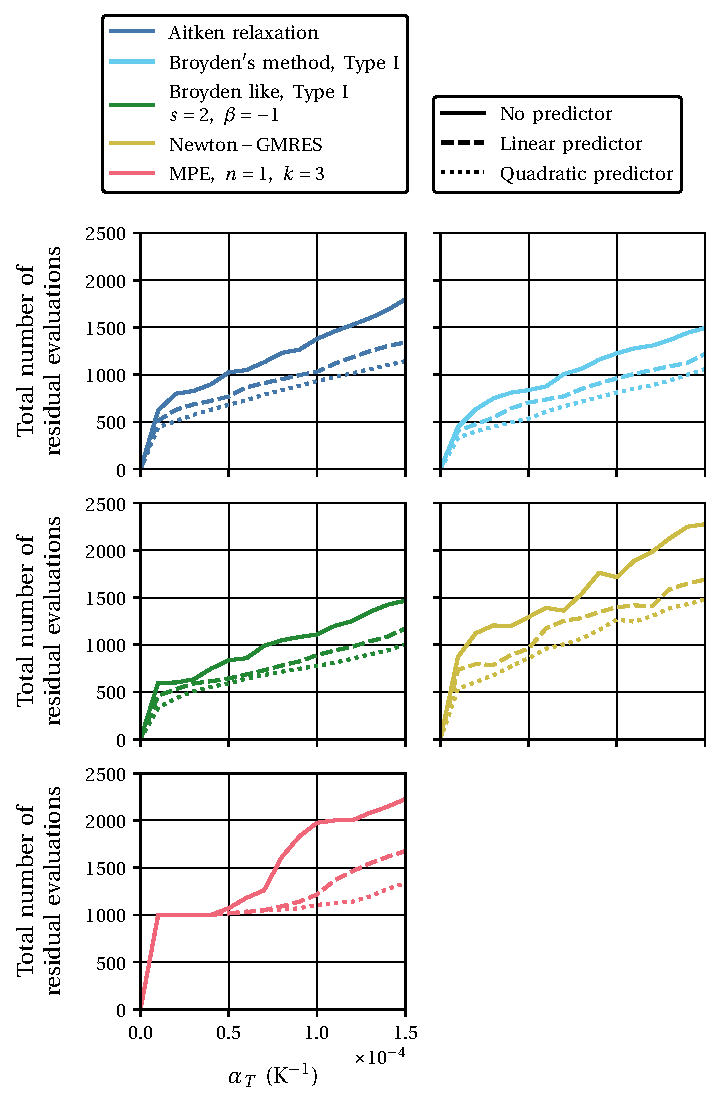
\includegraphics[width=.85\textwidth]{thick_cylinder_comparison_best_pred_total_iters_coupl_strength_quad4fbar_pred.pdf}
 \caption{Total number of iterations as a function of the thermal expansion coefficient for the  best performing implicit methods in each class considered using a linear, a quadratic, and no predictor in the solution of the necking of a circular bar with \(\alpha_T=\SIrange{0}{1.5e-4}{\kelvin^{-1}}\) and \(\dot u_0 =\SI{0.5}{\milli\meter\second^{-1}}\).}
\label{fig:thick_cylinder_comparison_best_pred_total_iters_coupl_strength_quad4fbar_pred.pdf}
\end{figure}

\FloatBarrier

\pagebreak

\section{Necking of a circular bar}
\label{sec:mech-driv-probl}

The second validation example consists of the thermally triggered necking of a circular bar, as initially reported in \cite{simo_associative_1992} and replicated in \cite{danowski_computational_2014}.
The problem consists of a cylindrical bar of radius $r=\SI{6.413}{\milli\meter}$ and length $h=\SI{53.334}{\milli\meter}$ subject to a prescribed axial displacement $\bar{u}_{y}=\SI{8}{\milli\meter}$ at both ends during $t=\SI{8}{\second}$.
The supports at the tips allow transverse contraction of the specimen.
The bar is initially at the ambient temperature $T_{0}=T_{\infty}=\SI{293}{\kelvin}$ and is subject to heat transfer by convection at all boundaries, with a heat transfer coefficient $h_{c} = \SI{17.5e-3}{\newton\per\milli\meter\per\second\per\kelvin}$.
The material is modeled with the constitutive model by \cite{simo_associative_1992} and the material properties are given in Table~\ref{tab:matpropsnecking}.
%
\begin{table}
 \centering
 \caption{Material properties and initial and boundary conditions for the problem concerning the quasi-static finite strain thermo-elastic expansion of an infinitely long thick-walled cylinder.}
\label{tab:matpropsnecking}
 \begin{tabular}{lccS[exponent-mode=engineering]}
 \multicolumn{3}{l}{Material Properties} & {\vphantom{\Big |}Effective value}\\
 \hline\hline
 \vphantom{\Big |}Density & \(\rho\) & (\si{\newton\second^2\milli\meter^{-4}}) & 7.8e-9\\
 \vphantom{\Big |}Bulk modulus & \(\kappa\) & (\si{\newton\milli\meter^{-2}}) & 164206\\
 \vphantom{\Big |}Shear modulus & \(\mu\) & (\si{\newton\milli\meter^{-2}}) & 801938\\
 \vphantom{\Big |}Conductivity & \(k\) & (\si{\newton\second^{-1}\kelvin^{-1}}) & 45\\
 \vphantom{\Big |}Heat capacity & \(C_V\) & (\si{\milli\meter^2\second^{-2}\kelvin^{-1}}) & 460e6\\
 \vphantom{\Big |}Coefficient of thermal expansion & \(\alpha_T\) & (\si{\kelvin^{-1}}) & 10e-6\\
 \vphantom{\Big |}Dissipation factor & \(\chi\) & (-) & 900e-3\\
 \vphantom{\Big |}Initial yield stress at \(T_0\) & \(\sigma_{y,0}\) & (\si{\newton\milli\meter^{-2}}) & 450\\
 \vphantom{\Big |}Linear hardening coefficient at \(T_0\) & \(H\) & (\si{\newton\milli\meter^{-2}}) & 129.24\\
 \vphantom{\Big |}Saturation exponent & \(\delta\) & (-) & 16.93\\
 \vphantom{\Big |}Saturation yield stress at \(T_0\) & \(\sigma_{y,\infty}\) & (\si{\newton\milli\meter^{-2}}) & 715\\
 \vphantom{\Big |}Thermal softening parameter (\(\sigma_{y,0}\)) & \(\omega_0\) & (\si{\kelvin^{-1}}) & 2e-3\\
 \vphantom{\Big |}Thermal softening parameter (\(\sigma_{u,\infty}, H\)) & \(\omega_h\) & (\si{\kelvin^{-1}}) & 2e-3\\
 \hline
 \multicolumn{3}{l}{Boundary Conditions\vphantom{\Big |}} & \\\hline
 \vphantom{\Big |}Radius of the cylindrical bar & \(r\) & (\si{\milli\meter}) & 6.413\\
 \vphantom{\Big |}Length of the cylindrical bar & \(h\) & (\si{\milli\meter}) & 53.334\\
 \vphantom{\Big |}Maximum displacement at both ends & \(\bar u_y\) & (\si{\milli\meter}) & 8\\
 \vphantom{\Big |}Time to maximum displacement & \(t\) & (\si{\second}) & 8\\
 \vphantom{\Big |}Heat transfer coefficient & \(h_c\) & (\si{\newton\milli\meter^{-1}\kelvin^{-1}}) & 17.5e-3\\
 % \multicolumn{3}{l}{\vphantom{\Big |}All mechanical degrees of freedom fixed in the \(y\)- and \(z\)-directions.}\\
 \hline
 \multicolumn{3}{l}{Initial Conditions\vphantom{\Big |}} & \\\hline
 Initial temperature & \(T_0\) & (\si{\kelvin}) & {293}\\
 \hline
 \multicolumn{3}{l}{Reference value \vphantom{\Big |}} & \\\hline
 \vphantom{\Big |}Temperature at outer radius (\(r=r_0\)) & (\si{\kelvin}) & \\
 \hline\hline
 \end{tabular}
\end{table}

%
This classical benchmark in isothermal elastoplasticity renders a bifurcation problem where a geometric imperfection typically triggers the necking phenomenon.
In the thermomechanical version, the combination of plastic dissipation in the bulk and heat transfer at the boundaries produce a temperature field that becomes progressively more heterogeneous during the loading.
With growing elongation, the temperature rise in the center of the bar will increase relative to the exterior boundary and automatically trigger the necking, even for a geometrically perfect setup.

The problem is analyzed using two-dimensional axisymmetric QUAD4 elements for both the mechanical and the thermal problems.
Figure~\ref{fig:necking} illustrates the problem setup, the finite element mesh employed in the 2D simulations, and distinct stages of deformation and temperature field during the prescribed elongation, evidencing the significant necking of the bar.
%
\begin{figure}[p]
 \centering
 \def\svgwidth{1.0\linewidth}
 \footnotesize
 \input{figures/necking2.pdf_tex}
 \caption{Description of the thermally triggered necking of a circular bar problem, characteristic deformation, and temperature field stages during the loading and example axisymmetric finite element mesh. The results have been obtained with QUAD4 elements, non-adiabatic boundary conditions, the inconsistent mechanical dissipation formulation, and the Fourier law based on constant $k_{0}$.}
 \label{fig:necking}
\end{figure}
%
Only one-quarter of the specimen is simulated, resulting in a finite element mesh with 1326 nodes and 1250 elements.
Except where explicitly indicated, this is the mesh employed.
The load is applied in 80 equal time steps $\Delta t = \SI{0.1}{\second}$.
Using a backward Euler integration, a quasi-static solution is computed for the mechanical problem. The transient temperature field is integrated with the generalised-$\alpha$ method with $\rho_{\infty, T}=1.0$.

\subsection{Validation of the Numerical Results}

As validation for the results presented in the present work, the reaction force at the supports and the neck surface temperature at point A are compared to results found in the literature, see \ref{fig:necking}.
Different reference data is included in the analysis, particularly the adiabatic and non-adiabatic results presented in the original work by \cite{simo_associative_1992}, and the non-adiabatic results presented in \cite{danowski_computational_2014}.
It should be remarked that there are five fundamental differences between these two publications that lead to distinct results.
First, in \cite{simo_associative_1992}, the authors adopt a mechanical dissipation term that is thermodynamically inconsistent, based on the previously mentioned dissipation factor, $\chi$, whereas, in \cite{danowski_computational_2014}, the authors use the mechanical dissipation coming directly from the second law of thermodynamics.
Second, \cite{danowski_computational_2014} also uses a consistent structural heating term for the Gough-Joule effect, accounting for both elastic and plastic contributions.
In contrast, \cite{simo_associative_1992} considered the elastic contributions, exclusively.
For more information on the previous classification and mathematical formulas for the heating parcels, the reader is referred to \ref{cha:simo-miehes-thermo}.
The third difference is linked to the heat conduction law employed in each contribution.
Although the large deformation version of the Fourier law underlies both publications, \cite{simo_associative_1992} considered as a fixed material parameter the spatial thermal conductivity, $k$, and in \cite{danowski_computational_2014}, the material thermal conductivity, $k_{0}$, was instead interpreted as the fixed material parameter.
Without further mention, the latter is employed in the current work.
Fourth, \cite{simo_associative_1992} solved the coupled problem using an operator split scheme and \cite{danowski_computational_2014} pursued a monolithic solution.
Last, regarding  spatial discretisation, \cite{danowski_computational_2014} used HEXA8-FBAR elements and \cite{simo_associative_1992} employed mixed displacement-pressure QUAD8 elements.

To enable a fair comparison with the reference data, the numerical solution is calculated using both the adiabatic and non-adiabatic setups.
Furthermore, consistent and inconsistent interpretations are considered in the latter, including a calculation with fixed $k$.
The evolution of the reaction force and neck surface temperature as a function of the prescribed displacement are shown in \ref{fig:necking-results} for the 2D and 3D solutions, respectively.
\begin{figure}[!p]
 \centering
 % \includegraphics[width=1.0\linewidth]{./solution-techniques-thermomechanics/figures/necking/necking_results.pdf}
 \caption{evolution of the reaction force at the tips of the bar and the neck surface temperature with the prescribed displacement using QUAD8 elements with reduced integration (QUAD8R) and HEXA8-FBAR elements.}
 \label{fig:necking-results}
\end{figure}
%
From a physical interpretation standpoint, the plot of reaction forces suggests that the simulation occurs almost entirely in the elastoplastic regime.
The necking process does not occur in the isothermal and adiabatic solutions, with the adiabatic solution predicting slightly smaller reactions due to the thermal softening effect.
Also, in this case, the temperature evolves uniformly in the bar and grows nearly linearly over time, as captured in the numerical solutions.
As previously postulated, the necking is automatically triggered in the non-adiabatic solutions, which produces a heavy reduction in the reaction force starting approximately at $\bar{u}_{y}=\SI{4}{\milli\meter}$, followed by a steep temperature rise due to the higher plastic dissipation.

Inspecting \ref{fig:necking-results} from a validation perspective, the numerical results show a good agreement with the literature.
The correlation between the non-adiabatic, inconsistent solution and fixed $k$ with the results from \cite{simo_associative_1992} is very satisfactory, both on the temperature and the reaction force side.
Curiously, while the reaction force seems almost insensitive to the element type employed, the neck temperature is better approximated with the QUAD8 solution, especially near the maximum displacement.
The slight difference between these cases can presumably be attributed to the distinct element technology and coupling solution strategy used to obtain the two curves.
Relative to the solutions based on the consistent mechanical heating, the numerical results show good agreement with the curves extracted from \cite{danowski_computational_2014} up to $\bar{u}_{y}=\SI{3}{\milli\meter}$, but features significant differences from there on, both in the mechanical and thermal responses.
The results are consistent insofar as the numerical solution obtained predicts a smaller temperature increase but larger reaction forces, as the thermal softening is less pronounced.
Unfortunately, to the author's knowledge, no other bibliographical sources consider the entirely consistent thermomechanical version of the model to support any of the sides.
Nevertheless, as the accuracy relative to the results from \cite{simo_associative_1992} is already adequate, the possibly remaining issue resides at the constitutive model level and therefore does not compromise the coupling environment.
It should also be remarked that if the prescribed displacement is slightly larger, the weakly coupled partitioned solution diverges at some point.
This can be expected from the mathematical properties of this type of strategy, as discussed in this chapter.
In truth, numerical divergence can be observed to start near $\bar{u}_{y}=\SI{8}{\milli\meter}$ for the non-adiabatic, inconsistent solution, see \ref{fig:necking-results}.
In principle, it is possible to stabilize the solution by employing more advanced techniques, for instance, implicit coupling strategies with numerical acceleration.
Despite being paramount for a robust computer simulation tool, these topics are postponed to future developments.
Overall, the present results are a sound indication of the correct implementation of the coupling environment, particularly the data exchange and solution orchestration.
\begin{figure}
% 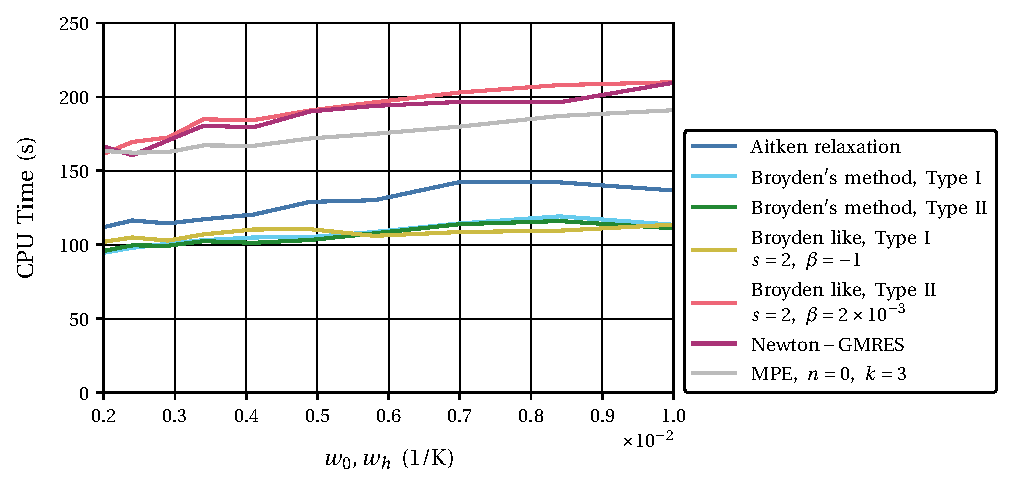
\includegraphics[width=.85\textwidth]{necking_comparison_methods_best_cpu_time_coupl_strength_quad4fbar_pred}
\end{figure}

\begin{figure}
% 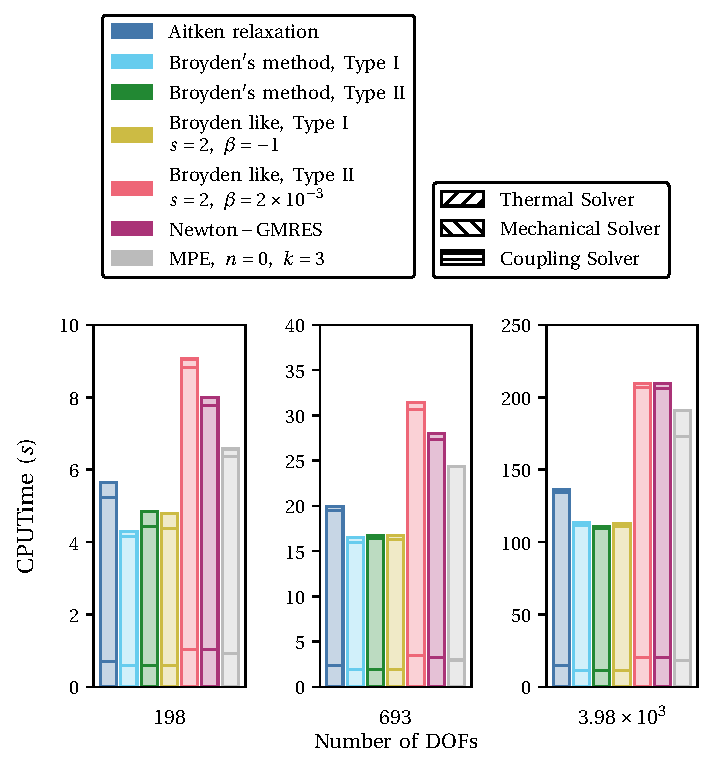
\includegraphics[width=.85\textwidth]{necking_comparison_methods_best_time_profile_mesh_size_quad4fbar_pred}
\end{figure}

\FloatBarrier

\subsection{Evaluation and comparison of implicit solution methods for the coupled problem}

The following contains the results concerning the evaluation and comparison of the implicit solution methods for coupled problems considered in this work.
The discussion starts with the methods that require only one evaluation of the residual, implicitly requiring the solution of both the thermal and the mechanical problems by the corresponding solvers per nonlinear iteration.
The Broyden-like family of methods fall into this category too but are considered by themselves and are presented next.
The Newton-Krylov methods are also analyzed, followed by the vector extrapolation methods in cycling mode.
The discussion ends with a comparison of the best methods in each class.

As for the thermoelastic case, the analysis presented is based mainly on three pieces of information.
The first concerns how the residual evolves as a function of the nonlinear iterations.
The second is the number of function evaluations needed to solve the coupled problem to the desired accuracy at each time step.
The third is the total number of residual evaluations needed to solve the coupled problem to the desired accuracy as a function of the thermal softening parameters, \(w_0\) and \(w_h\), set to be equal.
The larger the softening parameters \(w_0\) and \(w_h\), the stronger the coupling between the thermal and mechanical fields, and the more challenging the problem is to solve.

The maximum displacement at both ends is restricted to \SI{5}{\milli\meter} applied in \SI{5}{\second} to prevent an excessive elongation of the elements in finite element simulation that often leads to simulation failure.
The thermal softening parameters \(w_0=w_h\) vary from \SIrange{2e-3}{1e-2}{\kelvin^{-1}}, such that the larger the thermal softening parameters \(w_0\) and \(w_h\), the stronger the coupling.
This can be understood from Figure~\ref{fig:necking_single_iter_diff_w_0_n_iter_time_quad4fbar_pred}.
In this case, it shows the total number of residual evaluations corresponding to the total number of nonlinear iterations as a function of the thermal softening for the fixed-point method.
As \(w_0\) increases, the displacement at which the coupling is the most substantial moves to the left, and the width of the corresponding peak gets larger, employing a stronger coupling.

\begin{figure}[htbp]
 \centering
 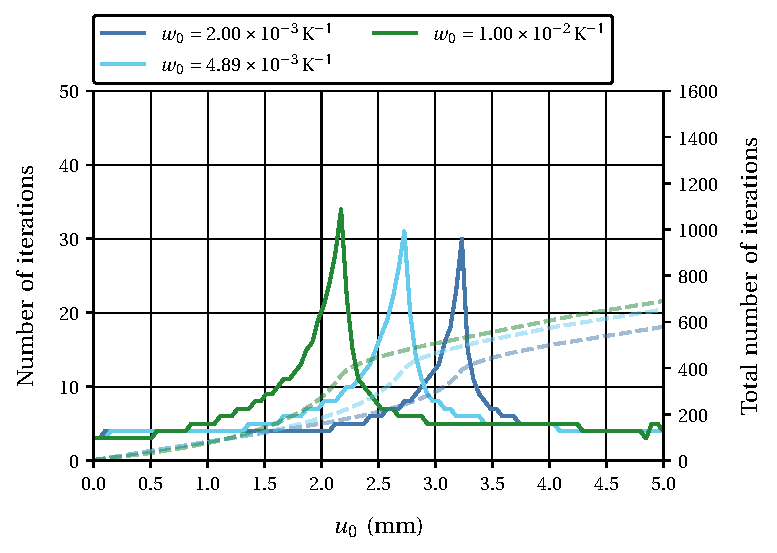
\includegraphics[width=.85\textwidth]{necking_single_iter_diff_w_0_n_iter_time_quad4fbar_pred}
 \caption{Total number of residual evaluations as a function of the thermal expansion coefficient for the fixed-point method in the solution of the necking of a circular bar with \(w_0=w_h=\SIlist{2e-3; 4.89e-3; 1e-2}{\kelvin^{-1}}\).}
\label{fig:necking_single_iter_diff_w_0_n_iter_time_quad4fbar_pred}
\end{figure}

\subsubsection{Methods with only one residual evaluation per iteration}

The methods with only one residual evaluation per nonlinear iteration considered are the fixed-point method (see Section~\ref{sec:fixed_point_approach}), the underrelaxation method (see Section~\ref{sec:underrelaxation}), the Aitken relaxation (see Section~\ref{sec:aitken_relaxation}) and Broyden's method, Type I and II (see Section~\ref{sec:multisecant}).
These are, a priori, the most economical methods regarding residual evaluations, as only one is performed per nonlinear iteration.
The underrelaxation is performed with \(\omega = 0.5\), and the first relaxation coefficient for the Aitken relaxation is also set to 0.5.

Figure~\ref{fig:necking_single_iter_n_iter_time_quad4fbar_pred} presents the number of nonlinear iterations/residual evaluations needed to solve the coupled thermomechanical problem at each time step and the total (cumulative) number of iterations needed with \(w_0=w_h=\SI{1e-2}{\kelvin^{-1}}\).
It is clear from the number of nonlinear iterations needed to solve the problem at \(u_y\approx\SI{2.3}{\milli\meter}\) that the coupling is the strongest at this moment.
It corresponds to the moment where the necking of the bar begins.
There is a marked performance difference between the methods under analysis, with the Broyden methods taking much fewer iterations, 10, than either the Aitken relaxation, 18, or the fixed-point method, 34.
For all other moments, the performance of the implicit methods under analysis is very similar, except for the under relaxation.
This behavior is probably due to the poor choice of the relaxation coefficient.

\begin{figure}[htbp]
 \centering
 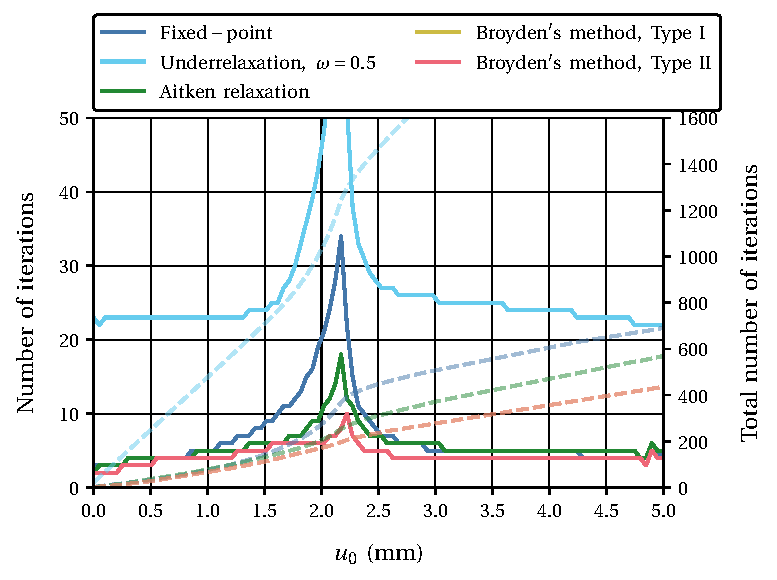
\includegraphics[width=.85\textwidth]{necking_single_iter_n_iter_time_quad4fbar_pred}
 \caption{number of nonlinear iterations needed to solve the coupled problem at each time step and the total number of iterations needed to solve the coupled problem for the implicit methods that perform only one evaluation per nonlinear iteration in the solution of the necking of a circular bar with \(w_0=w_h=\SI{1e-2}{\kelvin^{-1}}\).}
\label{fig:necking_single_iter_n_iter_time_quad4fbar_pred}
\end{figure}

Figure~\ref{fig:necking_single_iter_n_iter_coupl_strength_quad4fbar_pred} presents the total number of residual evaluations, in this case, corresponding also to the total number of nonlinear iterations, as a function of the thermal softening parameters, which control the strength of the coupling between the thermal and the mechanical fields, respectively.
The most efficient methods are the two Broyden methods, followed by the Aitken relaxation.
The difference between the total number of iterations is around 100 for the three different methods.

\begin{figure}[htbp]
 \centering
 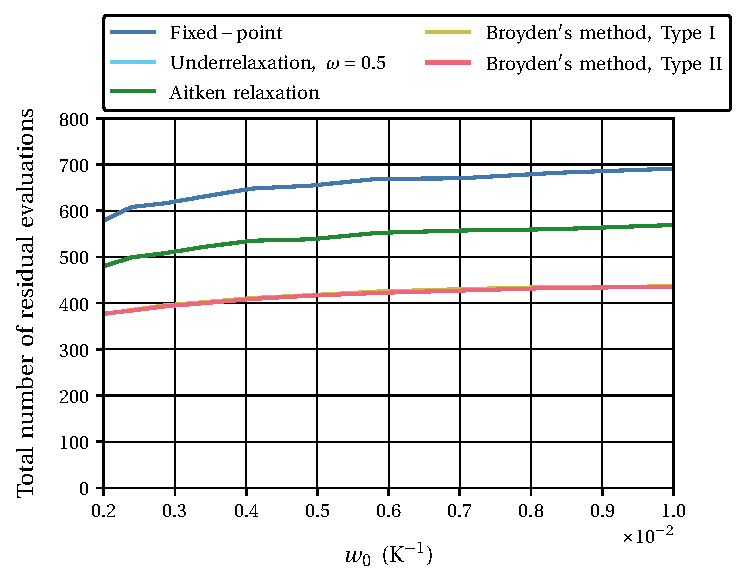
\includegraphics[width=.85\textwidth]{necking_single_iter_n_iter_coupl_strength_quad4fbar_pred}
 \caption{Total number of residual evaluations as a function of the thermal expansion coefficient for the implicit methods that perform only one evaluation per nonlinear iteration in the solution of the necking of a circular bar with \(w_0=w_h=\SIrange{2e-3}{1e-2}{\kelvin^{-1}}\).}
\label{fig:necking_single_iter_n_iter_coupl_strength_quad4fbar_pred}
\end{figure}

\FloatBarrier

\subsubsection{Broyden-like method}

The Broyden-like methods considered (see Section~\ref{sec:multisecant}) employ as group sizes \(s=1,\ 2,\ 3,\ 6\) with a maximum number of previous iterations available equal to 6.
The mixing parameters considered are \(\beta=-1,\ \num{2e-3},\ \num{2e-2}\).
All combinations are also considered with both Type I and Type II updating for the approximation to the Jacobian.

Figures~\ref{fig:necking_broyden_like_type_i_n_iter_time_quad4fbar_pred} and \ref{fig:necking_broyden_like_type_ii_n_iter_time_quad4fbar_pred} present the number of nonlinear iterations/number of function evaluations needed to solve the coupled problem at each time step and the total (cumulative) number of iterations needed in the solution of the necking of a circular bar with \(w_0=w_h=\SI{1e-2}{\kelvin^{-1}}\).
Regarding the methods using \(\beta=-1\), the difference between Type I and II methods is not noticeable.
However, the different size groups lead to different behaviors.
A larger group size leads to worse results for the displacement values where the coupling is the weakest.
On the other hand, the number of iterations where the coupling is the strongest are about the same for all group sizes.
For \(\beta=\num{2e-3}\) and \num{2e-2} the only group size that converges is \(s=6\).
For the other group sizes, the simulation breaks down approximately after reaching \(u_y=\SI{2.3}{\milli\meter}\).
This failure happens because the mechanical solver fails with an exploding residual in its internal Newton-Raphson procedure.
It doesn't seem to be directly related to the coupling solver itself.

\begin{figure}[htbp]
 \centering
 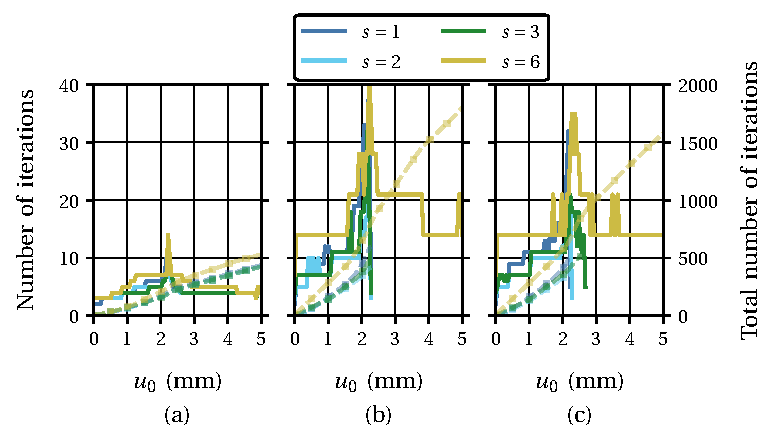
\includegraphics[width=.85\textwidth]{necking_broyden_like_type_i_n_iter_time_quad4fbar_pred}
 \caption{
Number of nonlinear iterations needed to solve the coupled problem at each time step and the total number of iterations needed to solve the coupled problem for Broyden-like methods with Type I update and group sizes \(s=1\), 2, 4 and 6: (a) \(\beta=-1\), (b) \(\beta=\num{2e-3}\), and (c) \(\beta=\num{2e-2}\) in the solution of the necking of a circular bar with \(w_0=w_h=\SI{1e-2}{\kelvin^{-1}}\).}
\label{fig:necking_broyden_like_type_i_n_iter_time_quad4fbar_pred}
\end{figure}

\begin{figure}[htbp]
 \centering
 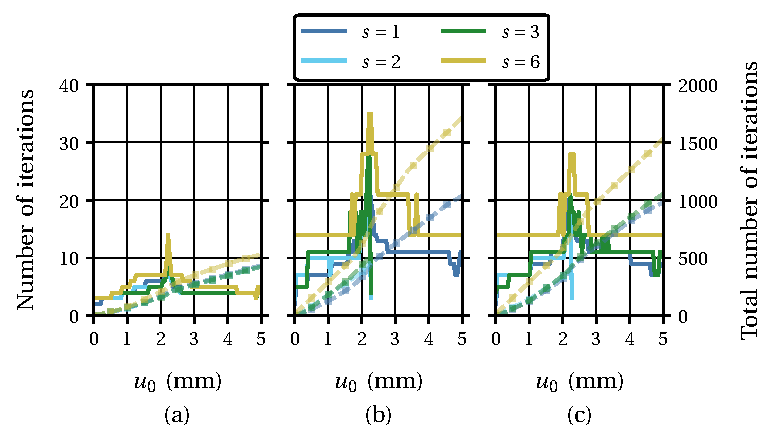
\includegraphics[width=.85\textwidth]{necking_broyden_like_type_ii_n_iter_time_quad4fbar_pred}
 \caption{Number of nonlinear iterations needed to solve the coupled problem at each time step and the total number of iterations needed to solve the coupled problem for Broyden-like methods with Type II update and group sizes \(s=1\), 2, 4 and 6: (a) \(\beta=-1\), (b) \(\beta=\num{2e-3}\), and (c) \(\beta=\num{2e-2}\) in the solution of the necking of a circular bar with \(w_0=w_h=\SI{1e-2}{\kelvin^{-1}}\).}
\label{fig:necking_broyden_like_type_ii_n_iter_time_quad4fbar_pred}
\end{figure}

Figures~\ref{fig:necking_broyden_like_type_i_n_iter_coupl_strength_quad4fbar_pred} presents the total number of residual evaluations as a function of the thermal softening parameter, respectively, for the Broyden-like methods with Type I update considered.
The same results are presented in Figures~\ref{fig:necking_broyden_like_type_ii_n_iter_coupl_strength_quad4fbar_pred} for the Broyden-like methods with Type II update.
For \(\beta=-1\), the best results are obtained for \(s=\SIlist{1; 2; 3}{}\).
However, convergence is not always achieved for \(s=3\).
For \(\beta=\num{2e-3}\) and \num{2e-3} the best results seem to be obtained for \(s=2\) when the methods do converge.
However, this is a rare occurrence.

\begin{figure}[htbp]
 \centering
 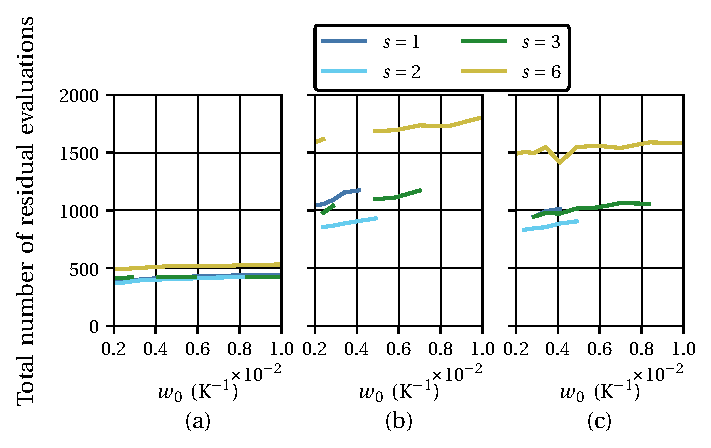
\includegraphics[width=.85\textwidth]{necking_broyden_like_type_i_n_iter_coupl_strength_quad4fbar_pred}
 \caption{Total number of residual evaluations as a function of the thermal expansion coefficient for the implicit methods for Broyden-like methods with Type I update and group sizes \(s=1\), 2, 4 and 6: (a) \(\beta=-1\), (b) \(\beta=\num{2e-3}\), and (c) \(\beta=\num{2e-2}\) in the solution of the necking of a circular bar with \(w_0=w_h=\SIrange{2e-3}{1e-2}{\kelvin^{-1}}\).}
\label{fig:necking_broyden_like_type_i_n_iter_coupl_strength_quad4fbar_pred}
\end{figure}

\begin{figure}[htbp]
 \centering
 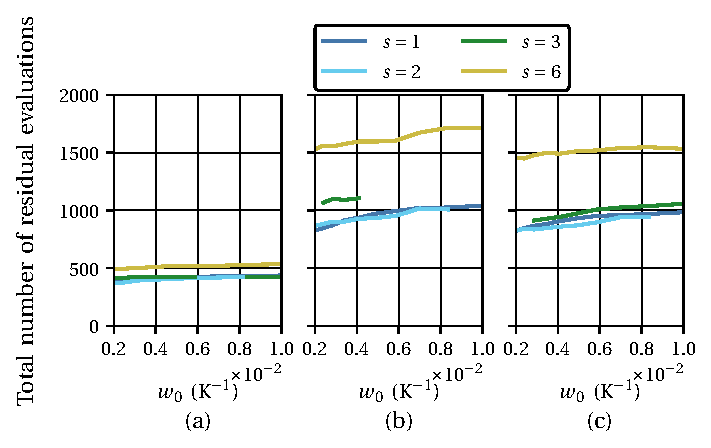
\includegraphics[width=.85\textwidth]{necking_broyden_like_type_ii_n_iter_coupl_strength_quad4fbar_pred}
 \caption{Total number of residual evaluations as a function of the thermal expansion coefficient for Broyden-like methods with Type II update and group sizes \(s=1\), 2, 4 and 6: (a) \(\beta=-1\), (b) \(\beta=\num{2e-3}\), and (c) \(\beta=\num{2e-2}\) in the solution of the necking of a circular bar with \(w_0=w_h=\SIrange{2e-3}{1e-2}{\kelvin^{-1}}\).}
\label{fig:necking_broyden_like_type_ii_n_iter_coupl_strength_quad4fbar_pred}
\end{figure}

\FloatBarrier

\subsubsection{Newton-GMRES method}

The Newton-Krylov method examined here uses as the Krylov subspace solver the GMRES method (see Section~\ref{sec:newton_krylov}).
Different forcing terms are employed.
The values considered are \(\eta=\num[print-unity-mantissa=false]{e-1}\), \num[print-unity-mantissa=false]{e-3} and \num[print-unity-mantissa=false]{e-5}.
The Eisenstat-Walker scheme for the adaptive choice of the forcing term is also utilized.

Figure~\ref{fig:necking_newton_krylov_n_iter_time_quad4fbar_pred} presents the number of nonlinear iterations needed to solve the coupled problem at each time step and the total (cumulative) number of iterations needed.
For the Newton-GMRES methods considered, the moment where the coupling is the strongest is not as clear as for the methods considered until now.
However, the number of iterations needed to solve the thermomechanical problem at each timestep is the largest for \(u_y = \SI{2.3}{\milli\meter}\).
Also, contrary to the other methods, where the coupling is the weakest, there is still some difference between the methods considered.
In general, higher forcing terms lead to fewer iterations.
However, remember that less iteration doesn't necessarily correspond to fewer residual evaluations.

\begin{figure}
 \centering
 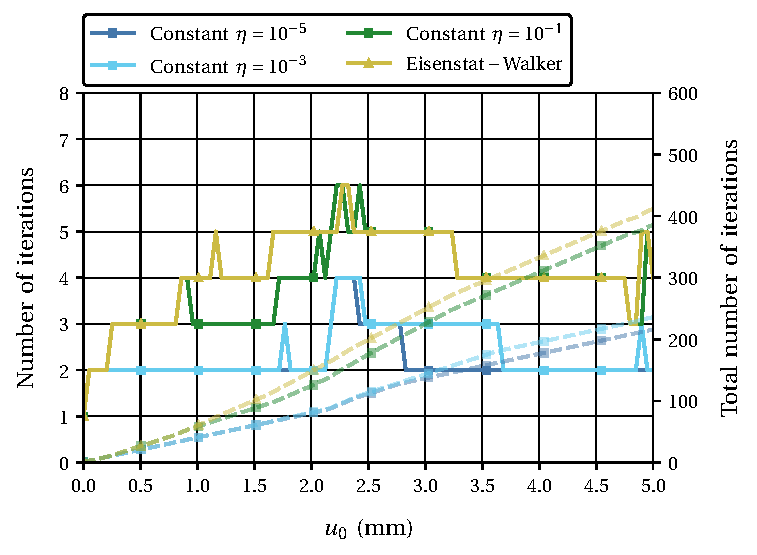
\includegraphics[width=.85\textwidth]{necking_newton_krylov_n_iter_time_quad4fbar_pred}
 \caption{Number of nonlinear iterations needed to solve the coupled problem at each time step and the total number of iterations needed to solve the coupled problem for the Newton-GMRES method with a constant forcing term (\(\eta=\num{1e-5},\ \num{1e-3},\ \num{1e-1}\)) and the Eisenstat-Walker scheme in the solution of the necking of a circular bar with \(w_0=w_h=\SI{1e-2}{\kelvin^{-1}}\).}
\label{fig:necking_newton_krylov_n_iter_time_quad4fbar_pred}
\end{figure}

Figure~\ref{fig:necking_newton_krylov_n_iter_coupl_strength_quad4fbar_pred} present the total number of residual evaluations as a function of the thermal softening parameters \(w_0\) and \(w_h\).
The best performing method employs a constant forcing term equal to \num{1e-3}.
The other constant forcing terms and the Eisenstat-Walker method display a similar efficiency.
The methods using a constant forcing also fail to converge for \(w_0=w_h=\SI{2e-3}{\kelvin^{-1}}\).

\begin{figure}
 \centering
 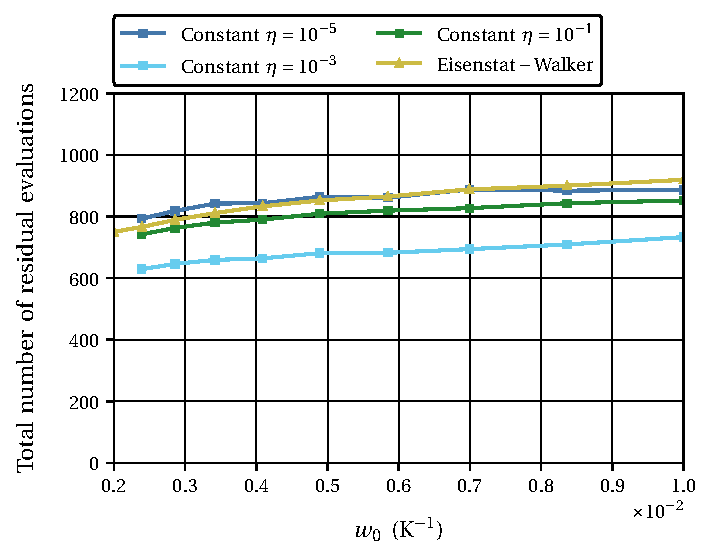
\includegraphics[width=.85\textwidth]{necking_newton_krylov_n_iter_coupl_strength_quad4fbar_pred}
 \caption{Total number of residual evaluations as a function of the thermal expansion coefficient for the Newton-GMRES method with a constant forcing term (\(\eta=\num{1e-5},\ \num{1e-3},\ \num{1e-1}\)) and the Eisenstat-Walker scheme in the solution of the necking of a circular bar with \(w_0=w_h=\SIrange{2e-3}{1e-2}{\kelvin^{-1}}\).}
\label{fig:necking_newton_krylov_n_iter_coupl_strength_quad4fbar_pred}
\end{figure}

\FloatBarrier

\subsubsection{Polynomial vector extrapolation in cycling mode}

The polynomial vector extrapolation methods in cycling mode considered are the MPE and RRE, restricted to at most five evaluations of the residual function per nonlinear iteration.
Thus, the combinations analyzed are characterized by the ordered pairs \((n,k)=(1,1)\), \((1,2)\), \((1,3)\), \((2,1)\), \((2,2)\) and \((3,1)\).

Figure~\ref{fig:necking_extrap_pol_n_iter_time_quad4fbar_pred} presents the number of residual evaluations needed to solve the coupled problem at each time step and the total (cumulative) number of iterations needed with \(w_0=w_h=\SI{1e-2}{\kelvin^{-1}}\).
There is no clear difference between the MPE and the RRE.
The moment of strongest coupling is visible for the methods using few residual evaluations per nonlinear iteration, such as \((n,k)=(1,1)\).
For \((n,,k)=(1,3)\), this is much less noticeable.
Regarding the moments where the coupling is weaker, the difference between the methods is less marked.

\begin{figure}[htbp]
 \centering
 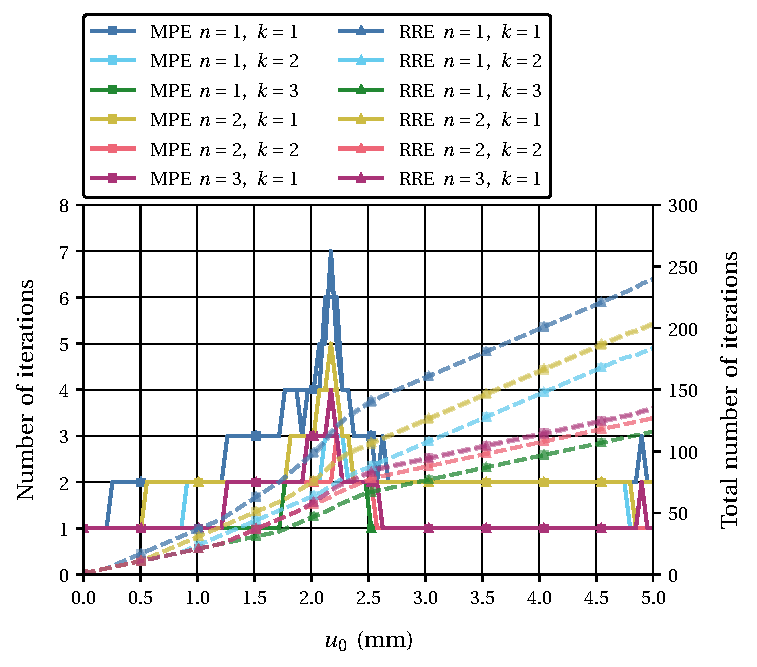
\includegraphics[width=0.9\textwidth]{necking_extrap_pol_n_iter_time_quad4fbar_pred}
 \caption{number of nonlinear iterations needed to solve the coupled problem at each time step and the total number of iterations needed to solve the coupled problem for the polynomial vector extrapolation methods in cycling mode, MPE and RRE, restricted to at most five evaluations of the residual function per nonlinear iteration in the solution of the necking of a circular bar with \(w_0=w_h=\SI{1e-2}{\kelvin^{-1}}\).}
\label{fig:necking_extrap_pol_n_iter_time_quad4fbar_pred}
\end{figure}

Figures~\ref{fig:necking_extrap_pol_n_iter_coupl_strength_quad4fbar_pred} present the total number of residual evaluations as a function of the thermal expansion coefficient.
The method which performs the best uses \((n,k)=(1,3)\).
The second and third best methods are also the ones using five residual evaluations per nonlinear iteration, \((n,k)=(2,2)\) and \((n,k)=(3,1)\).

\begin{figure}[htbp]
 \centering
 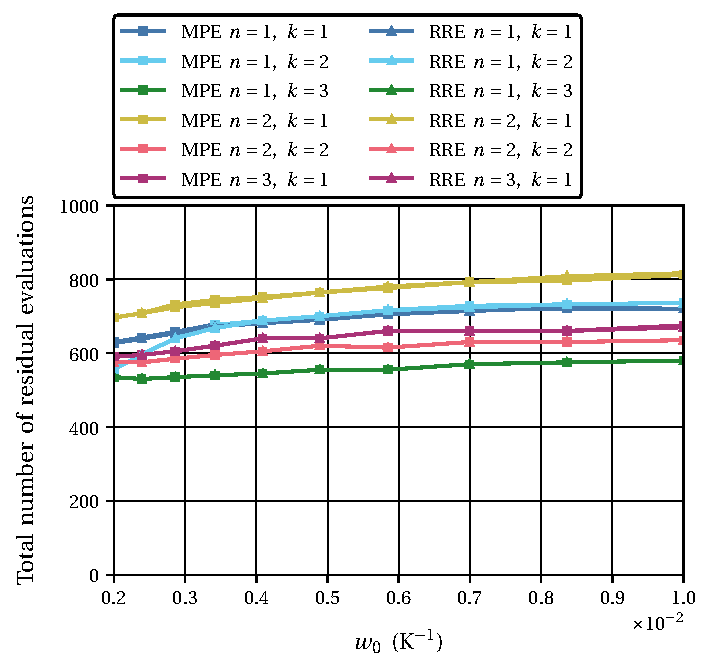
\includegraphics[width=0.9\textwidth]{necking_extrap_pol_n_iter_coupl_strength_quad4fbar_pred}
 \caption{Total number of residual evaluations as a function of the thermal expansion coefficient for the polynomial vector extrapolation methods in cycling mode, MPE and RRE, restricted to at most five evaluations of the residual function per nonlinear iteration in the solution of the necking of a circular bar with \(w_0=w_h=\SIrange{2e-3}{1e-2}{\kelvin^{-1}}\).}
\label{fig:necking_extrap_pol_n_iter_coupl_strength_quad4fbar_pred}
\end{figure}

\FloatBarrier

\subsubsection{comparison of the best methods in each class}

In this section, the best-performing methods from each of the classes considered are compared with each other.
The implicit methods selected are Aitken relaxation, Broyden's method with Type I update, a Broyden-like method with \(\beta=-1\) and \(s=2\), the Newton-GMRES method with \(\eta=\num{e-3}\) and the MPE in cycling mode with \((n,k)=(1,3)\).

Figure~\ref{fig:necking_comparison_best_cpu_time_n_iter_coupl_strength_quad4fbar_pred} shows the total CPU time in seconds and the total number of residual evaluations as a function of the thermal softening parameters for the best performing implicit methods in each class considered.
The best performing methods are Broyden's and the Broyden-like methods, whose performance is very similar.
They are followed by the Aitken relaxation and the MPE in cycling mode, also displaying a comparable efficiency.
The Newton-GMRES method is the worse performing method considered.
As the thermal softening parameters, and thus the strength of the coupling, increase, all the methods display approximately a similar loss in efficiency.
Table~\ref{tab:necking_res_cpu_nr_func_best} surmises all the results previously discussed regarding the computational time each solvers takes.

\begin{figure}[hbtp]
 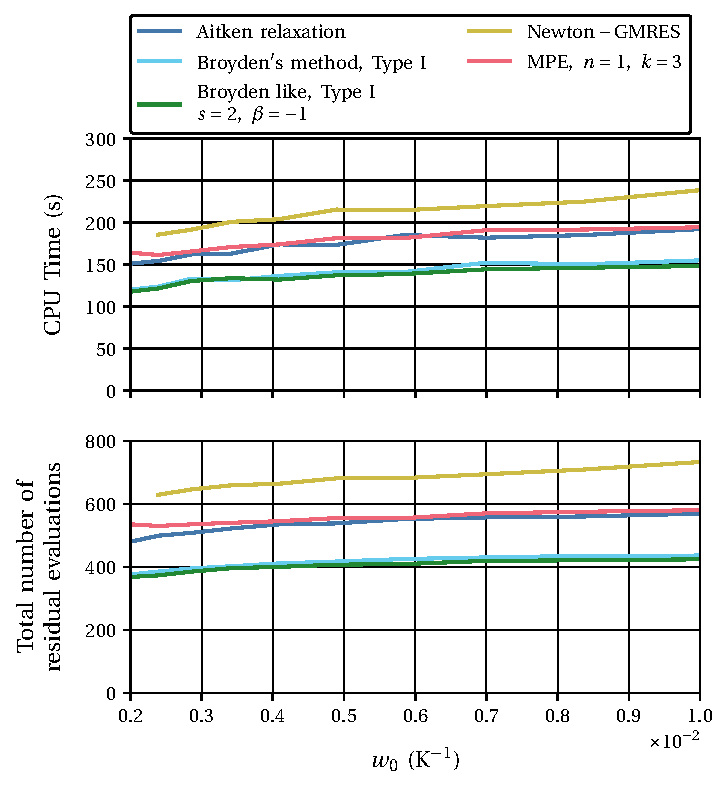
\includegraphics[width=.85\textwidth]{necking_comparison_best_cpu_time_n_iter_coupl_strength_quad4fbar_pred}
 \caption{Total CPU time in seconds and the total number of residual evaluations as a function of the thermal softening parameters \(w_0=w_h\) for the best performing implicit methods in each class considered in the solution of the necking of a circular bar with \(w_0=w_h=\SIrange{2e-3}{1e-2}{\kelvin^{-1}}\).}
\label{fig:necking_comparison_best_cpu_time_n_iter_coupl_strength_quad4fbar_pred}
\end{figure}

\begin{table}[hbtp]
 \centering
 \caption{Total CPU time in seconds and the total number of residual evaluations as a function of the thermal softening parameters \(w_0=w_h\) for the best performing implicit methods in each class considered in the solution of the necking of a circular bar with \(w_0=w_h=\SIlist{2e-3; 4.89e-3; 1e-2}{\kelvin^{-1}}\).}
 \label{tab:necking_res_cpu_nr_func_best}
 % \setlength{\tabcolsep}{3pt}
 \begin{tabular}
 {l
 S[round-mode=places, round-precision=2, table-format = 1.2e1]
 S[round-mode=places, round-precision=2, table-format = 1.2e1]
 S[round-mode=places, round-precision=2, table-format = 1.2e1]
 S[round-mode=places, round-precision=0, exponent-mode=fixed, fixed-exponent=0, table-number-alignment = center, table-format = 4.0]
 S[round-mode=places, round-precision=0, exponent-mode=fixed, fixed-exponent=0, table-number-alignment = center, table-format = 4.0]
 S[round-mode=places, round-precision=0, exponent-mode=fixed, fixed-exponent=0, table-number-alignment = center, table-format = 4.0] }
 \vphantom{\Big \vert}&  \multicolumn{3}{c}{CPU Time (\si{\second})} & \multicolumn{3}{c}{Nr Residual Evaluations} \\
 \cmidrule(lr){2-4}\cmidrule(lr){5-7}
 \vphantom{\Big \vert}\makecell[c]{$w_0$\\ (\SI[exponent-mode=input]{1e-3}{\kelvin^{-1}})} & {2} & {4.89} & {10} & {2} & {4.89} & {10}\\
 \hline\hline
 \vphantom{\Big \vert} AITK  & 1.51000e+02 & 1.73300e+02 & 1.92100e+02 & 4.80000e+02 & 5.38000e+02 & 5.69000e+02\\
 \vphantom{\Big \vert} BRDI  & 1.20100e+02 & 1.40700e+02 & 1.54900e+02 & 3.76000e+02 & 4.17000e+02 & 4.36000e+02\\
 \vphantom{\Big \vert} BRDI2  & \cellcolor{gray}1.17700e+02 & \cellcolor{gray}1.37100e+02 & \cellcolor{gray}1.48200e+02 & \cellcolor{gray}3.68000e+02 & \cellcolor{gray}4.07000e+02 & \cellcolor{gray}4.24000e+02\\
 \vphantom{\Big \vert} NEWT  & NC & 2.15400e+02 & 2.38500e+02 & 4.36000e+02 & 7.81000e+02 & 8.33000e+02\\
 \vphantom{\Big \vert} MPE  & 1.64100e+02 & 1.81300e+02 & 1.94300e+02 & 5.35000e+02 & 5.55000e+02 & 5.80000e+02\\

 \hline\hline
 \end{tabular}
\end{table}

\subsubsection{Effect of predictiors}

Figure~\ref{fig:necking_comparison_best_pred_total_iters_coupl_strength_quad4fbar_pred} presents the effect of employing a linear or quadratic predictor on the number of residual evaluations needed to fully solve the thermomechanical problem under analysis as a function of the thermal expansion coefficient.
All methods improve using the polynomial predictors, with the best effects being achieved using the quadratic predictor.
The decrease in residual evaluations is around 30\% to 40\% for all methods using the quadratic predictor, except for the MPE.
The polynomial vector extrapolation method displays a much smaller increase in efficiency from the polynomial predictors considered.
Finally, the use of predictors allows the Newton-GMRES method to converge for \(w_0=w_h=\SI{2e-3}{\kelvin^{-1}}\).

\begin{figure}[hbtp]
 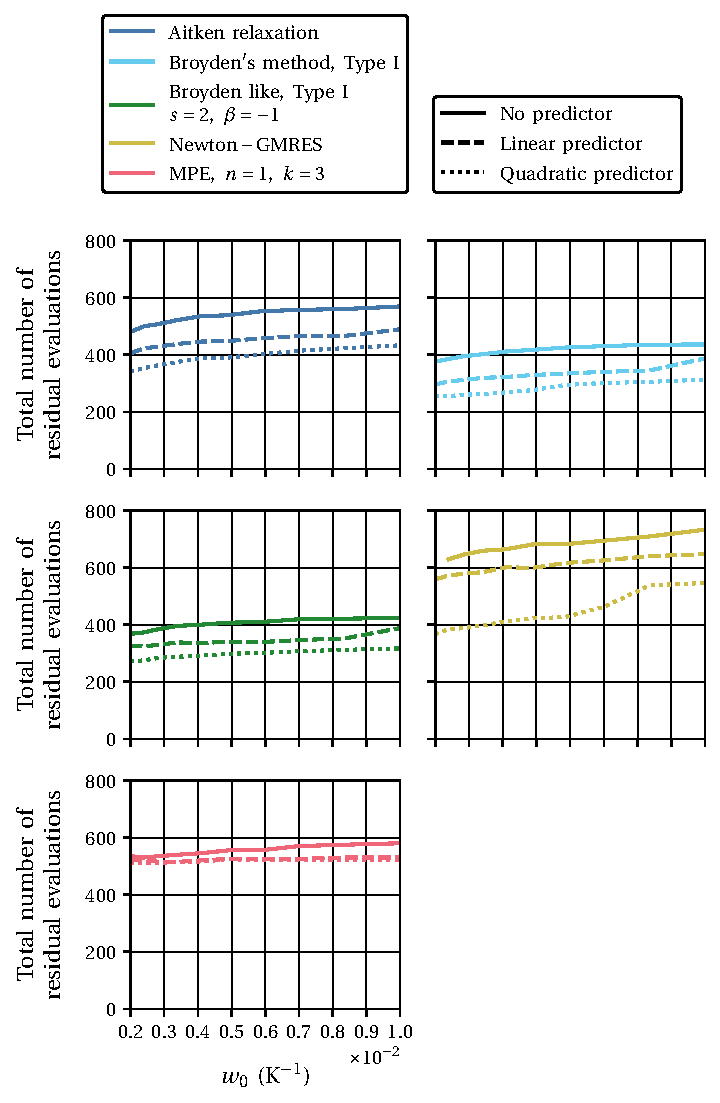
\includegraphics[width=.85\textwidth]{necking_comparison_best_pred_total_iters_coupl_strength_quad4fbar_pred}
 \caption{Total number of iterations as a function of the thermal softening parameters \(w_0=w_h\) for the best performing implicit methods in each class considered using a linear, a quadratic, and no predictor in the solution of the necking of a circular bar with \(w_0=w_h=\SIrange{2e-3}{1e-2}{\kelvin^{-1}}\).}
\label{fig:necking_comparison_best_pred_total_iters_coupl_strength_quad4fbar_pred}
\end{figure}


\section{Conclusions}

Given the set of numerical results shown, Broyden-like techniques with \(\beta=-1\), \(s=1\), which is also Broyden's method, and \(s=2\), both with Type I update appear to be the most advantageous methods in terms of computational effort.
The Aitken relaxation is also effective, particularly for the thermoelastic problem.
It requires the least amount of memory and is the easiest to implement.
The MPE in cycling mode with \((s,k)=(1,3)\) competes with the Aitken relaxation for the thermo-elastoplastic problem, but is more comparable to the Newton-GMRES with \(\eta=\num{1e-3}\) for the thermoeleastic problem.
Among the techniques deemed the best in each class, the last one performs the poorest.
However, because the Jacobian of the residual is well estimated, it is the approach that most easily accepts global strategies such as line search.
The requirement for a global strategy isn't illustrated in the problems described, but it may be significant in other circumstances.
Last but not least, the polynomial predictors significantly increased computing effectiveness without adding to the complexity of the numerical methods.

\FloatBarrier
